\documentclass{UoNMCHA}

% Packages to include
\usepackage[square,sort,comma,numbers]{natbib}%\usepackage[authoryear]{natbib}
\usepackage{array,booktabs} % For nice tables
\usepackage{amsmath,amsfonts,amssymb,mathrsfs,bm} % For nice 
\usepackage{color}
\usepackage{enumerate}
\usepackage{listings}
\usepackage{subfig}
\usepackage{hyperref}
\usepackage[normalem]{ulem}
\usepackage[parfill]{parskip}   % For replacing paragraph indenting with a newline instead

\usepackage{csvsimple} % For tables from CSV
\usepackage{float} % Used for forcing diagrams to the [H] action


\usepackage[shortlabels]{enumitem} % Custom lists

\usepackage{stringstrings}      % Sentence Case
\usepackage[explicit]{titlesec} % Sentence Case

% \usepackage{dirtytalk} % \say

\usepackage{caption}

% Wikipedia-style "citation needed" macro source: https://gist.github.com/martinarroyo/b9e0a963ad27169a6eee
\newcommand{\citationneeded}{\textsuperscript{\color{blue} [citation needed]}}
% New macro to make defining labels easier.
\newcommand{\flagforreview}{\textsuperscript{\color{red} [FLAGGED FOR REVIEW]}}
\newcommand{\rephrase}{\textsuperscript{\color{red} [REPHRASE?]}}

\newcommand{\inlineQuote}[1]{`` #1 ''}

\newcommand{\fancyquote}[1]{\begin{quotation}\inlineQuote{#1}\end{quotation}}
\newcommand{\fref}[1] {Figure \ref{#1}}
\newcommand{\sref}[1] {Section \ref{#1}}
\newcommand{\tref}[1] {Table \ref{#1}}
\newcommand{\aref}[1] {Appendix \ref{#1}}
\newcommand{\lref}[1] {Listing \ref{#1}}

\newcommand{\fFigure}[3]{
	%\begin{minipage}%[H] %figure is a floating page, consider replacing with   
        \begin{center}  
            \includegraphics[width=#3\linewidth]{Figures/#1}  
        \captionof{figure}{#2}
            \label{#1}
        \end{center}
	%\end{minipage}
}

% \newcommand{\NewSection}[1]{
%     \clearpage 
%     \section{#1}
% }

% \newcommand\SentenceCase[1]{%
%   \caselower[e]{#1}%
%   \capitalize[q]{\thestring}%
% }
% \titleformat{\section}
%   {\normalfont\Large\bfseries}{\thesection}{1em}{\SentenceCase{#1}\thestring}

% \newcommand{\SentenceCaseSubSection}[1]{\subsection{\SentenceCase{#1}}}
% \newcommand{\SentenceCaseSubParagraph}[1]{\subparagraph{}{\SentenceCase{#1}}}

 

%\LoadClass[twoside,a4paper,11pt]{scrartcl}

% Make all math bigger
%\setmathfont{XITS Math}[10pt,version=xits]

%\defaultscriptratio=0.7

% Number equations per section
\numberwithin{equation}{section}

\hypersetup{
%    bookmarks=true,         % show bookmarks bar?
%    unicode=false,          % non-Latin characters in AcrobatÕs bookmarks
%    pdftoolbar=true,        % show AcrobatÕs toolbar?
%    pdfmenubar=true,        % show AcrobatÕs menu?
%    pdffitwindow=false,     % window fit to page when opened
%    pdfstartview={FitH},    % fits the width of the page to the window
    pdftitle={Chris Caelli | FYP Part B Report},    % title
    pdfauthor={Chris Caelli},     % author
    pdfsubject={FYP PART B},   % subject of the document
%    pdfcreator={Creator},   % creator of the document
%    pdfproducer={Producer}, % producer of the document
%    pdfkeywords={keyword1} {key2} {key3}, % list of keywords
%    pdfnewwindow=true,      % links in new window
    colorlinks=true,       % false: boxed links; true: colored links
    linkcolor=blue,          % color of internal links
    citecolor=blue,        % color of links to bibliography
%    filecolor=magenta,      % color of file links
    urlcolor=blue           % color of external links
}

\definecolor{MATLABKeyword}{rgb}{0,0,1}
\definecolor{MATLABComment}{rgb}{0.1328125,0.54296875,0.1328125}
\definecolor{MATLABString}{rgb}{0.625,0.125,0.9375}

\lstset{language=Matlab,
    basicstyle=\small\ttfamily,
    keywordstyle=\color{MATLABKeyword},
    %identifierstyle=,
    commentstyle=\color{MATLABComment},
    stringstyle=\color{MATLABString},
    numberstyle=\tiny,
    %numbers=left,
    basewidth=0.5em}




\firstpage{1}    % Set page number for first page
\UoNMCHAreportNo{MECH4841 Part B} %Report number
\UoNMCHAyear{2019}   % Year
\shorttitle{FYP Report - CCAELLI} %For odd pages
%%%%%%%%%%%%%%%%%%%%%%%%%%%%%%%%%%%%%%%%%%%%%%%%%%%%
\begin{document}
\title{The effect of supplementary data on acoustic event classification through machine learning \\ \ \\
{\small Final Year Project Report - MECH4841 Part B  \\JUNE 2019}}
\author[UoNMCHA]{Christopher Caelli}
\address[UoNMCHA]{
Student of Mechatronics Engineering,\\
The University of Newcastle, Callaghan, NSW 2308, AUSTRALIA \\
% Student Number: 3206246 \\
E-mail: \href{mailto:Christopher.Caelli@uon.edu.au}{\textsf{Christopher.Caelli@uon.edu.au}}}
%%%%%%%%%%%%%%%%%%%%%%%%%%%%%%%%%%%
\maketitle
\onecolumn

\vspace{-5mm}
\section*{Mandatory Dot Point Summary}
\vspace{-3mm}

check all flagforreview \flagforreview \\
check all citationneeded \citationneeded \\
Tense: Past, Future etc. Search "was", "is" "ed" etc.
Check contraction. it's, don't etc.
check for our, we, I, they're, your, you, etc.
check for st-ray - inca-se the-y block sh-t
check ref and replace with fref, tref, aref etc.
fix header to og %School of Engineering, Discipline of Mechanical Engineering and Mechatronics
check \\refs\{\} for whether the fullstop is before or after
review the use of section vs paragraph vs subsection etc.
sklearn vs scikit-learn.
check for bad refs by ? ?? ??? ????

As per the FYP Handbook: \\
I did:
\begin{itemize}
    \item I learnt and prototyped two machine learning solutions that takes audio and physical data (GPS, accelerometer, gyroscope) to compare whether the supplementary data could improve the classification of an acoustic event, as measured by the F1 score.
    \item I learnt and prototyped a pipeline to record data, process it, classify it, and output it.
    \item I used my mechatronics subject matter learnings to best apply machine learning to this problem. This includes Mechatronics Design (trade off and evaluations from MCHA3000), sound pre-processing, preprocessing Inertial Measuring Unit data, and how Audio waveforms can be treated as energy, and statistics from MECH2450/MCHA3900. \flagforreview
    \item I learnt and used system engineering techniques to elicit requirements from my university and work stakeholders
    \item I managed and worked with another employee to implement a proof of concept app to record data as an input into this project. This involved using my software engineering skills and project management skills to create a schema, develop the android app, and present it to the relevant stakeholders. \rephrase
\end{itemize}


%    \item 
%     \item \sout{I helped integrate this proof of concept with a larger C\# replay system at my work. This involved lat/long coordinate calculations for display playback, leading the configuration management with a local git server, and helping develop the data pipeline where the proof of concept feeds through my machine learning classifier, and into the larger replay system.}

\newpage

%%%%%%%%%%%%%%%%%%%%%%%%%%%%%%%%%%%
\vspace{-5mm}
\section*{Executive summary}
\vspace{-3mm}
The project investigated whether supplementary data (Accelerometer, Gyroscope, GPS) will improve a classifiers ability to classify an "acoustic event" in an acoustic event detection / classification (AED/C) problem. The motivation behind this was to improve AED/C without onerous microphone requirements, to enable more widespread commercial use of AED/C. \\

\sref{sec:ProblemAnalysis} of the project begins by evaluating the research problem for a car use case, and eliciting the design requirements through system engineering principles. \\

\sref{sec:LitReview} reviews current research. Presently the field is expanding with broader advances in the wider machine learning community, however AED/C remains a non-trivial problem that doesn't have a viable solution yet. Comparatively to the wider machine learning community, acoustic event detection is very limited in active researchers. This specific issue hasn't been explicitly answered. \\

\sref{sec:Method} details the method of selecting the desired output, the required data input, a metric to score by, a classifier, optimising hyperparameters against the previous options, and finally training and validating against the data. For this project:
{\small
\begin{itemize}
    \item The desired output is a label (or labels) detailing the acoustic event in the sample (e.g. The labels found in \aref{apx:ExtraSensoryLabels} like `Walking').
    \item The required data is the ExtraSensory dataset, or a custom dataset as recorded by the project's App.
    \item The score selected is the F1 score. This is due to it being an industry standard.
    \item The classifier chosen is the MLPClassifier which is a feedforward neural network, trained via backpropagation.
    \item Hyperparameters of the MLPClassifier are chosen via a Random Search Cross Validation.
    \item Training and Validation was run with Early Stopping using a 10\% validation set, using 59 out of the 60 ExtraSensory users.
    \item Final testing is done with the 60\textsuperscript{th} user.
\end{itemize}

\sref{sec:Results} the desired results are a 10.5\% and 11.9\% relative improvement in F1 score for a Binary and Multi-label classifier respectively. This is calculated through analysis of F1 Scores of a binary MLPClassifier, and a multi-label MLPClassifier, both trained on the ExtraSensory dataset using the method described in \sref{sec:Method}. The output of the classifiers are also analysed and found to be valid classifiers for real-world use. \flagforreview

\sref{sec:Discussion} evaluates and discusses limitations of the results. It will discuss how multi-sensor AED/C is effective but requires more datasets to test smaller, more specific tasks. \flagforreview It also discusses why the result will be valid in other projects.

\sref{sec:Conclusion} will present how these results will contribute to the field

\sref{sec:futurework} will list future work into new datasets with a greater number of labels, and further work into specifics of the result. \rephrase
% This document will cover the author's progress through the Final Year Project. The scope of the project is a portable data recording system coupled with offline processing to track and identify specific physical events in close proximity that occurred during recording. acoustic event detection and classification is the focus of this paper, and the goal of this FYP report is exploring and validating current research techniques in an uncontrolled environment for a specific use case. The content of this paper will start with, system engineering, problem analysis, a review into the current research and will expand to document python implementation, machine learning, data pre-processing, app development and progress in developing the proof of concept to take logged data from a phone and process it on a sever to create a “trackfile” (special csv file).
\newpage
%%%%%%%%%%%%%%
\vspace{-2mm}
\section*{Acknowledgements}
\vspace{-3mm}
I'd like to thank my partner Brigid for encouraging and supporting me throughout this project. \\

I'd also like to thank each and every mechatronics Academic staff member at the University of Newcastle . The teaching staff care about their students, and I want that to grow.
% My Mechatronics experience 
\newpage
\tableofcontents
\newpage
%%%%%%%%%%%%%%%%%%%%%%%%%%%%%%%
\clearpage \section{Introduction}
 
The mobile phone is an omnipresent force in modern society with the number of unique mobile phone users reached 5.1 billion at the end of 2018 \cite{GSMA}. Every phone carries a microphone, and in a data intensive field such as machine learning, there is an untapped potential for these 5.1 billion microphones. %for public and private good remain a heated debate.

% * Introduce field
% * discuss what the current work is like in field, what current results are, maybe what can be determined from data presently etc
% * What is the problem/question
% * nitty gridd of the debrief problem?
% * Why does my question help solve this problem/answer this question

\subsection{Machine Learning Field}
The machine learning field dates back to the first attempted reproduction of a neuron network \cite{mcculloch1943logical} in an attempt to explain the physical decision making process of the nervous system.

Significant scientific papers on machine learning from mathematicians and early computer scientists ... through the late 20th century.

The advent of cheaper, and faster processing power has revived the idea of machine learning, and the widespread availability of data has against furthered the boom.

Machine learning concerns itself with any application of a computer learning to complete a task.

\paragraph{Learning Computers}
Machine learning is based on the concept of having a computer \inlineQuote{learn}. This broad term has been used to described fitting a function to historical data, iterative output optimisation based on previous hypothesis, and 'genetic algorithms' which are a random search, using previous success as an initial guess for a new random guess.

All these strategies have a common theme: machine learning rewards progress and punishes mistakes. Often, but not always, this can be reduced down to a cost/constraint model.

\paragraph{Signal Processing}
Signal Processing is a field of mathematics focused on the use, interpretation, creation and modification of time varying structures of information. The broad definition of a signal could be anything from a wave of light, to a graph of house prices. This project will be primarily concerned with the physical phenomenon of vibrations of varying amplitude, known as audio.

\paragraph{Audio Signal Processing}
Audio (or acoustic) signal processing is the sub field of signal processing that is the focus of this report. Audio signal processing is an old field (dating back to the 17th century), and looks to understand the science behind an audio signal, and the many applications of it. 

\subparagraph{Music}
% From the ancient human reproduction of music from a memory of musical signal, to musical notation to spread a musical signal, to devices with a musical signal physically encoded onto it (such as a mu) for mechanical reproduction, to the disc record gramophones, to the 
Audio signal processing has been a key element of technological development in music. From human reproduction music instruments, to a wide range of mechanical analogue devices to record and reproduce sound, to finally a discretised digital signal. All these methods represent an audio signal, but the advent of a digital signal has allowed for the widespread use of digital signal processing in a wide range of applications.
For example; new musical effects, compression and storage, sound recognition, noise cancellation, equalisation. %all of these could be done anolg

\subparagraph{Acoustic Event}
Audio signals can encompass a wide medium of data. It can cover creative aspects such as music, but it can also capture certain "acoustic events". This could be any event that is measurable through audio. In some cases, an event could be inferred from the audio signal.

\subparagraph{New Opportunities}
Audio digital signal processing has allowed widespread application of actionable audio data. Speech recognition, speech synthesis, acoustic pattern detection, etc.

\subsection{Classification}
Classification is the process of determining, based on observations, what categories an item belongs in. This is a phenomenon present where there can be a ground truth of membership.
It is possible for categories to be mutually-exclusive, such as that of the an animal's genus, or it could be non-unique, such as a song's genre. It can also be the process of labelling a signal, such as whether an acoustic event was detected in an audio signal.

\paragraph{Current State of Acoustic Event Classification}
Presently the latest results from the field can be found in the Detection and Classification of
Acoustic Scenes and Events (DCASE) competitions. Presently, preliminary results from DCASE 2019's Task A challenge demonstrates an accuracy score ({\small }$ \frac{Correctly\;Classified\;Samples}{Total\;Samples} $}) \cite{Mesaros2018_DCASE}

\subsection{The Problem}
This project aims to answer the question: What is the effect of supplementary data on acoustic event classification through machine learning?. 

To do this, results will analyse the F1 Scores of a binary MLPClassifier, and a multi-label MLPClassifier, both trained on the ExtraSensory dataset using the method described in Section \ref{sec:Method}.
Additionally, the output of the classifiers will be analysed for \inlineQuote{validity}. Does the classifier successfully detect and classify an acoustic event?

The desired results are a demonstrable difference (or lack thereof) in the F1 score, after comparing a classifier with and without supplementary data.

\paragraph{Motivation for the Problem}
The capacity to identify a physical event in the real world using sound would open the door to a whole new realm of data. The potential implications and applications are limitless; assistance and reality closed captioning for the hearing impaired, improved security closed loop TV, increased transparency and documentation of a ride sharing trip, and early detection of potential accidents or medical emergencies to name a few. The primary focus of the new potential is to review AEC/D as a method of debriefing across multiple industries. \\

\subparagraph{Debreifing (or After Action Report)}

Debriefing is effectively an education tool used to educate an individual, a group or record a more holistic history of an event, for purposes of performance feedback \cite{recentAAR}.
%The After Action Report style of debriefing is one where an educator works with a student to go through the following steps: an explanation of an event, e, reporting of measures of performance, and/or opportunities to further investigate the results of a study, investigation, or assessment of performance after participation in an immersive activity is complete.
The formal debrief originated from the World War 2, with SLA Marshell's "interviews after combat" \cite{DebriefAAR}. Since then, the "After Action Report" was developed by the US Army as ...
\fancyquote{a professional discussion of an event, focused on performance standards, that enables soldiers to discover for themselves what happened, why it happened and how to sustain strengths and improve on weaknesses \cite{TC2520}.}
This is a key tool in training after any group activity, and has been extended to many industry, most notably in the training of Doctors \cite{johnson2011debriefing}.\flagforreview. Traditionally this is done through a collection of primary sources (where available) and secondary sources. In the information age, these primary sources have expanded to include large datasets, recordings and other digital forensics. This new and increasing range of primary sources provides the potential to significantly improve the steps of debriefing, and ultimately improve debriefing outcomes \cite{PsychologicalDebriefing2012}.




% of the form of an activation function (such as a sigmoid, ReLu, etc), can you \inlineQuote{optimise} it until it's function best fits a process model that identifies sounds?

% It is more broadly an aspect of artificial intelligence based on the idea that systems can learn from data, identify patterns and make decisions with minimal human intervention.
% This paper will report on the Author’s progress of harnessing this new potential and is organised as follows: \sref{sec:ProblemAnalysis} will discuss how the scope has been analysed and reduced, \sref{sec:LitReview} will review the literature of this research topic, \sref{sec:Method} will discuss the method of implementing the technology, \sref{sec:Results} will discuss the results, and \sref{sec:Discussion} will discuss the results of the proof-of-concept.

% To organise your introduction section you can use the following structure:
% \begin{itemize}
%     \item \textbf{Position}: Show there is a problem and that it is important to solve it.
%     \item \textbf{Problem}: Describe the specifics of the problem you are trying to address
%     \item \textbf{Proposal}: Discuss how you are going to address this problem. Use the literature to back-up your approach to the problem, or to highlight that what you are doing has not been done before
% \end{itemize}
% Here you need to sell why what you are doing is important, and what benefits will it bring if you are successful and solve the problem? 
%
\section{Background}

\subsection{Machine Learning}
A definition for Machine learning is taken from Tom M. Mitchell's 1997 textbook, \inlineQuote{machine learning}
\begin{quote}
    A computer program is said to learn from experience E with respect to some task T and some performance measure P, if its performance on T, as measured by P, improves with experience E \cite{Mitchell1997}.
\end{quote}

This definition of machine learning can be applied to this project; the task T (AED/C), the E (Audio, IMU, GPS), and P (a traditional F1 score). 

The computer program described in this project has been produced in Python, using the scikit-learn and TensorFlow libraries. \flagforreview

\paragraph{Machine Learning from a Mechatronics Perspective}
Machine learning was the focus of this report. Machine learning is a field of Engineering and Computer Science concerned with automating the discovery and modelling of a process. This process is usually a classification or regression function. In a nutshell, it is about training a computer algorithm to learn from data.\\

It's application in this report has parallels to a traditional optimisation problem in mechatronics: Given a \inlineQuote{plant} {\itshape(or, a neural network)}, how can someone \inlineQuote{optimise} {\itshape(train)} the plant's \inlineQuote{parameters} {\itshape(both weightings and hyperparameters)} as to \inlineQuote{minimise an error} {\itshape(or, maximise a classification/regression score)}?

\subsection{Key Concepts}

\paragraph{Traditional Machine Learning}
The traditional approach to machine learning has been to fit a function to a collection of historical samples, called a dataset.

\paragraph{Truth in Classification}
The process of machine learning relies on having examples of audio data (and supplementary data), paired with a true classification from that known data. This is what is more broadly known as a supervised learning task. A key concept for this project is to be comparing the classifier produced, against the recorded truth of the samples. This allowed the comparison of the classifier against 


%%%%%%%%%%%%%%%%%%%%%%%%%%%%%%%%%%%%%%%%%%%%%%%%%%%%%%%%%%%%%%%%%
\clearpage \section{Review of Literature}\label{sec:LitReview}
A literature review of the current research was conducted with guidance from University of Queensland’s guide to Literature reviews \cite{QueenslandReview}. There are 3 nested areas of research that are of interest to this project:
\begin{itemize}
    \item The wider classification and regression research topic
    \item The machine learning topic that covers many fields of implemented and theoretical machine learning applications
    \item The specific field of acoustic event detection and classification (AED/AEC) - this field has traditionally relied on older techniques, and is undergoing a revolution with machine learning. 
\end{itemize}

\fFigure{niche.png}{The literature for this project is a niche topic in the machine learning area of research}{0.8}


\subsection{Acoustic Event Detection and Acoustic Event Classification}
Historically the technologies for AED/AEC have been support vector machine (SVMs), Hidden Markov Models (HHMs), and more generally, digital signal processing (DSP) classifiers. In the last 8 years, AED and AEC research has been a popular emerging topic of research. Research has focused on the two key tasks: detection (when did an acoustic event occur in the audio, and when did it stop?) and classification (what sound occurred?). New research papers are often the result of Detection and Classification of Acoustic Scenes and Events Competitions (DCASE) competitions. DCASE is an official Institute of Electrical and Electronics Engineers (IEEE) Audio and Acoustic Signal Processing (AASP) competition. \fref{F1_score.png}.

\fFigure{F1_score.png}{Tampere University of Technology Researcher Toni Heittola's F1 Results reflect the AED/AEC field of research with drastic improvements over the last 8 years \cite{ToniWebsite}.}{0.8}

\subsection{Detection and Classification of Acoustic Scenes and Events Competitions (DCASE)}
The DCASE competitions format started 2013, had its second competition in 2016, and has been a yearly event since. Since 2017, there has been a new format where the competition starts march, formal results are released by September, and a workshop for participants on the best results in November \cite{2018Schedule}. 2016 was the first to feature machine learning (winning teams incorporated machine learning into ensemble model classifiers). By 2017 all entries utilised machine learning. The results from DCASE2018 indicate that progress in the AED/AEC field had allowed more sophisticated, real-world applications to be evaluated, such as DCASE2018's Challenge Task \#4 \cite{2018n}. This task focused on using a subset of Google's AudioSet to determine the audio class, and the timestamps of when that class occurred within a sample. The complexity of the dataset, the number of acoustic classes and fidelity of output were unprecedented in the AEC field. The winning results for this level of complexity did not score as high a F1 score compared to the DCASE2017 competition. DCASE2017 featured more controlled environments/datasets across the 4 tasks which likely resulted in the disparity (2017 had a 41.7\% F1 score \cite{2017results} vs 2018’s 32.4\% \cite{2018n}). It is however DCASE 2018 that presented the best precedent for the problem addressed in this paper.

\subsection{Leading Research, DCASE2018 Task 4 Winner}
The winning model used in the DCASE2018 Task 4 challenge used a “Mean-teacher” model for classification, a convolutional neural network (CNN) for context gating (a pre-classifier step to improve flaws in training methodologies for some machine learning models \cite{Yan16}) and a bidirectional recurrent neural network (RNN) to improve the utilisation of unlabelled, unbalanced training datasets \cite{winners}. The bidirectional RNN is an important would be an important element for this report if the AudioSet dataset was being used. This is because the leading dataset outside of DCASE challenges is the weakly labelled Google AudioSet, of which only small percentage of is balanced.

\begin{table}[h!]
    \begin{center}
        \caption{AudioSet data on cars}\label{tab:AudioSetCars}
        {\footnotesize
            \begin{tabular}{c l l l|}
                \hline\hline Dataset & Number of videos & Duration hours \\ \hline 
                Evaluation & 280 & 0.8 \\
                Balanced train & 296 & 0.8 \\
                Unbalanced train & 40,978 & 113.3 \\
                Overall & 41,554 & 114.9 \\
                \hline
            \end{tabular}
        }
    \end{center}
\end{table}
\begin{gather*}
    Car AudioSet:  \frac{0.8}{114.9}=0.69\%
\end{gather*}
%%%%%%%%%%%%%%%%%%%%%%%%%%%%%%%

\clearpage \section{Problem Analysis}\label{sec:ProblemAnalysis}

This project approached the problem through a system engineering perspective, a process which “is a structured and systematic methodology providing greater visibility and control over … new system[s]” \cite{limited2018systems}. This perspective was informed by ISO/IEC/IEEE 15288 \cite{IEEE15288} and Burge Hughes Walsh’s system engineering Toolbox \cite{SysThink2015}. The tools adapted and applied throughout this section are primarily derived from this \inlineQuote{System Engineering Toolbox}. 

% \subsection{Purpose of Problem Analysis} %should this be a 
The purpose of Problem Analysis is to define the scope of this project to be achievable, measurable and practical to implement. This took 2-4 weeks through June 2018, and remains an ongoing task. 

% \subsection{system engineering Tools for Problem Analysis}
The following system engineering tools have been adapted and implemented to develop this paper and the author’s understanding of the problem. 

\subsection{Current 18 Words}
A tool called \inlineQuote{18 Words} was used to constantly refine and maintain a description on the scope as it changed throughout problem analysis, with the intent to succinctly describe the project in \inlineQuote{close to 18 words}. The current “18 Words” is the following:\\
“The project aims to create a portable, trackfile recording system. This is coupled with offline processing to record specific physical events that occurred during recording.” 

\subsection{Tree Diagram}
With the understanding of what the project was intended to be, a Tree Diagram was drafted to explore missed requirements, hidden modules and other aspects of the project not yet considered. \fref{treeDiagram.png} shows a Tree Diagram breakdown for this FYP.

 \fFigure{treeDiagram.png}{A tree diagram for the project, used as a method of allocating work}{0.7}


\subsection{Quad of Aims}
The Quad of Aims is a tool used to explore 4 critical, high level aspects of the project as explained in \tref{tab:QuadOfAims}, and shown in \fref{QuadOfAims2.png}.

\fFigure{QuadOfAims2.png}{A Quad of Aims for the project might be A3 in size and would have the relevant information embedded. It may also be completed on a whiteboard.}{1}

 \begin{table}[h]
    \begin{center}
        \caption{Quad of Aims }\label{tab:QuadOfAims}
        {\footnotesize
            \begin{tabular}{c l l l|}
                \hline\hline Label & Description \\ \hline 
                Purpose & This is our “18 words” \\
                Stakeholders & University, Author’s Work \\
                Deliverables & Documentation, recommendations, FYP report, proof-of-concept \\
                Measure of Success & Review of Documentation by SMEs, review of FYP report, dry and wet run of proof-of-concept \\
                \hline
            \end{tabular}
        }
    \end{center}
\end{table}

This was done to evaluate any early risks, and the begin scope reduction on the project.

\subsection{Input Output Analysis}
The input output analysis of the system informed the bounds and requirements to operate the system. In this situation, it helped define the full scope of the project; including the technical and non-technical aspects of undertaking the MECH4841 Project as shown in \fref{InputOutput.png}.

\fFigure{InputOutput.png}{The input output analysis for the system}{0.75}


\subsection{Affinity Diagram}
An Affinity Diagram helped to add detail to the high level concepts in the project. There was a focus on putting tangible measurements onto requirements. During this process, system architecture decisions were made such as a trade review into online vs offline processing \aref{apx:TradeReview}, and subsequently splitting the system into smaller modules. The primary system had 2 key sub-systems: the recording system, and the offboard processing systems. An Affinity Diagram of the top-level system was created, and and this informed the creation of 2 affinity diagrams of the sub-systems. After this was complete, previous work was updated to reflect these changes. \fref{AffinityDiagram.png}.
\fFigure{AffinityDiagram.png}{The Affinity Diagrams for the full system architecture}{1}

\subsection{Systems Map}
A systems map uses the affinity diagram, input output analysis, and tree-diagram to identify the processes inside sub-modules that are needed to design the system. This was used to successfully \flagforreview to measure and estimate the workload necessary to implement data fusion alongside deep learning of acoustic classification and detection as shown in \fref{SystemMap.png}.
\fFigure{SystemMap.png}{A systems map for the project}{0.8}


\subsection{Sequence Diagram}
A Sequence Diagram was developed to analyse the flow of data through the processes identified in the System Map. This is shown in \fref{SequenceDiagram.png}. This helped to predict and manage any potential complexities and logistics related to the specific needs of each process. 
Originally, This Sequence Diagram was used to justify removing data fusion from the scope due to the large workload required to implement alongside machine learning. Later in the project, it was brought back into the scope of the project to help compare and evaluate its effectiveness in improving the overall system. 
\fFigure{SequenceDiagram.png}{A basic Sequence Diagram for the project}{0.7}


\subsection{N\textsuperscript{2} Analysis}
A N\textsuperscript{2} analysis methodically expands on the data flow within the system. This complimented the complexities highlighted in the sequence diagram by documenting what data was expected. A example of this is shown in \fref{n2analysis.png}
\fFigure{n2analysis.png}{A N\textsuperscript{2} Analysis for the project}{0.7}

\subsection{Spray Diagram}
The spray diagram shown in \fref{SprayDiagram.png} shows how details of the system could have multiple effects in design requirements, outcomes and operational use. Of interest in the diagram was the reciprocal relationship between high-quality output and high-quality input. The requirement of a high-quality output indicated the potential increase of production and design costs due to the necessitation of a high-quality input.

\fFigure{SprayDiagram.png}{A Spray Diagram for the project}{0.8}

\subsection{Matrix Diagram}
A matrix diagram was made to review reduced scope as shown in \fref{MatrixDiagram.png}. The numbers indicate \inlineQuote{packages of work}. By using a “strong”, “weak” or “none” indicator for each aspect of the project, each package of work was evaluated against it's likelihood to fulfill to the requirements of the project. It highlighted the difficulty in balancing the needs of both major stakeholders. 
\fFigure{MatrixDiagram.png}{A matrix diagram for the project}{0.8}

\subsection{Summary of Problem Analysis}
This section described the motivation for the project was applied AEC/D and this required scope reduction to ensure it was feasible as a Final Year Project. It also included a proof-of-concept machine learning solution within the scope. This should also provide an excellent learning opportunity for the author.

%%%%%%%%%%%%%%%%%%%%%%%%%%%%%%%%%%%%%%%%%%%%%%%%%%%%%%%%%%%%%%%%%%%%%%%%%%%%%%%%%%%%%%%%%%%%%%%%%%%%%%%%%%%%%%%%%%%
\clearpage \section{Method} \label{sec:Method}
\subsection{Introduction to the Method}
In a traditional machine learning problem there are 5 stages to the method: 
% list looks awful \flagforreview
\begin{enumerate}%[start=1,label={     Stage \arabic*:}]
    \item Data
    \item Preprocessing
    \item Model
    \item Fitting/Training
    \item Evaluation
\end{enumerate}

\citationneeded.

\subparagraph{Stage 1}
Stage 1 is choosing what raw data is available and what information the model must product. This is the inputs and the outputs that you want from the system, and the expected result.

\subparagraph{Stage 2}
Stage 2 is preprocessing. The purpose of preprocessing is to transform the available data into a format most appropriate for the intended analysis. This is inclusive of processes such as optimising, filtering, feature building\footnote{Producing refined data of interest to the model. For example, Mel-frequency cepstral coefficients (MFCCs) from raw Audio} and in many other options. Preliminary features are also evaluated in this stage to ascertain their quality and effectiveness in a preliminary model.

\subparagraph{Stage 3}
Stage 3 is selecting the model to be used. The selection of the model involves an understanding of what is best practice in the chosen topic area, a review of recent publications and their methods, and investigating if the chosen topic necessitates any special requirements. Once a model is elected, the parameters of the model must be determined (or evaluated) before a final model can be selected. This is done in the following two stages.

\subparagraph{Stage 4}
Stage 4 is fitting the model. The selected algorithm may need to be trained or fitted. This is the process of taking labelled input / output data (denoted as X, y) and supervising the model as it attempts to reproduce y from X. A common method to achieve this is through Stochastic Gradient Descent (SGD) and back propagation \cite{lecun2012efficient}. In summary, it is the process of changing the neuron weights proportionally to their contribution to the error. Equation \ref{eq:BP_grad_dec} adapted from \cite{lecun2012efficient} demonstrates this, where W is the machine learning weights for a given topology, $\eta$ is the proportional factor or step size, and the partial represents how each weight contributes to error.\\

\begin{gather}\label{eq:BP_grad_dec}
    W(t) = W(t-1) - \eta\frac{\partial E}{\partial W} 
\end{gather}
Once trained on a training set, the next stage is validating whether the model is sufficiently fit.

\subparagraph{Stage 5}
Stage 5 is validation. Validation is the process of checking the performance of the model against certain criteria. For instance, a model may be checked for overfitting, underfitting, bias, sensitivity, specificity, accuracy, precision, AUC (area under the (ROC) curve), and F1 score to name a few. F1 score was used as the primary measure in this project because the F1 has been used as a research industry standard for evaluating algorithms. \\

It is beneficial to work up methodically approach implementing machine learning. As each section will dramatically effect the next, care should be taken to optimise each stage before progressing in implementation. External to the method of building the machine learning classifier is the work involved in developing the pipeline associated with it. The main tasks to implement a machine learning classifier as a part of a larger solution are as follows:

\begin{itemize}
    \item Develop the use-case, and identify the output
    \item Investigate what data is available, and whether further data/datasets would be beneficial
    \item Choose a framework/technology to implement the machine learning algorithm in
    \item Build the machine learning classifier as described above, and test its effectiveness
    \item Validate the whole system by using the classifier in the pipeline (by taking the classified output, and appending it to the trackfile)
\end{itemize}

\subsection{Required Data}
The machine learning solution required GPS, accelerometer, gyroscope, and audio. A Google Pixel 2 was selected as the target data acquisition unit, which \tref{AndroidSensorsAvailable} below shows.
\begin{table}[h!] 
    \begin{center}
        \caption{Data Available \cite{pixelteardown}}\label{tab:AndroidSensorsAvailable}
        {\footnotesize
            \begin{tabular}{clll}
                \hline\hline Sensor & Description \\ \hline 
                GPS & The Pixel 2 uses the Snapdragon 835 System on Chip GPS receiver\\
                Accelerometer / Gyroscope & The Pixel 2 uses a Bosch BMI160 \\
                Audio & The Pixel 2 uses a Qualcom WCD9395 Audio Codec chip and a NXP TFA9891UK Audio Amplifier \\ \hline
            \end{tabular}
        }
    \end{center}
\end{table}

\subsection{Data Collection}

The decision of what data to collect and utilise was identified through the problem analysis in \sref{sec:ProblemAnalysis}. As the goal was to maximise the accuracy of the classifier (whilst still being an achievable goal), the data chosen for use and collection was GPS, accelerometer, gyroscope, and audio. As described in the problem analysis phase, the best platform for this would be a mobile phone as shown in \sref{sec:ProblemAnalysis} and \aref{apx:TradeReview}. 

\subsubsection{Project Android App}
Android was chosen as the platform as it had significant support for reading from the on-board sensors. The data available from the Android API can be seen in table \ref{tab:AndroidDataAvailable}. This was the source for accelerometer, gyroscope and GPS data. It was also selected due to its support for C/C++ through the Native Development Kit (NDK). The programming language C is required knowledge for many courses in the University of Newcastle Bachelor of Mechatronics degree. 


\begin{table}[h!]
    \begin{center}
        \caption{Data Available\citationneeded}\label{tab:AndroidDataAvailable}
        {\footnotesize
            \begin{tabular}{c l l l|}
                \hline\hline Sensor & Description \\ \hline 
                TYPE ACCELEROMETER & Acceleration force along the x axis (including gravity). \\
                 & Acceleration force along the y axis (including gravity). \\
                  & Acceleration force along the z axis (including gravity). \\
                TYPE ACCELEROMETER UNCALIBRATED & Measured acceleration along the X axis without any bias compensation. \\
                  & Measured acceleration along the Y axis without any bias compensation. \\
                  & Measured acceleration along the Z axis without any bias compensation. \\
                  & Measured acceleration along the X axis with estimated bias compensation. \\
                  & Measured acceleration along the Y axis with estimated bias compensation. \\
                  & Measured acceleration along the Z axis with estimated bias compensation. \\
                TYPE GRAVITY & Force of gravity along the x axis. \\
                 & Force of gravity along the y axis. \\
                 & Force of gravity along the z axis. \\
                TYPE GYROSCOPE & Rate of rotation around the x axis. \\
                  & Rate of rotation around the y axis. \\
                  & Rate of rotation around the z axis. \\
                TYPE GYROSCOPE UNCALIBRATED & Rate of rotation (without drift compensation) around the x axis. \\
                  & Rate of rotation (without drift compensation) around the y axis. \\
                  & Rate of rotation (without drift compensation) around the z axis. \\
                  & Estimated drift around the x axis. \\
                  & Estimated drift around the y axis. \\
                  & Estimated drift around the z axis. \\
                TYPE LINEAR ACCELERATION & Acceleration force along the x axis (excluding gravity). \\
                  & Acceleration force along the y axis (excluding gravity). \\
                  & Acceleration force along the z axis (excluding gravity). \\
                TYPE ROTATION VECTOR & Rotation vector component along the x axis (x  sin(o/2)). \\
                  & Rotation vector component along the y axis (y  sin(o/2)). \\
                  & Rotation vector component along the z axis (z  sin(o/2)). \\
                  & Scalar component of the rotation vector ((cos(o/2)).1 \\
                TYPE SIGNIFICANT MOTION & N/A \\
                TYPE STEP COUNTER & Number of steps taken by the user since the last reboot while the sensor was activated. \\
                TYPE STEP DETECTOR & N/A \\
                \\ \hline
            \end{tabular}
        }
    \end{center}
\end{table}

The app was developed over five weeks. It was able to record audio to a .wav file and record raw GPS data\footnote{Timestamps, latitude, longitude and altitude are recorded from the GPS sensor}, raw acceleration, and raw gyroscopic data. The output was an audio .wav file, and a Comma Separated Value (csv) file.

During this time, an Atlassian JIRA environment was set up to facilitate management (using concepts from ENG3500 - Project Management). The Atlassian "Git-Flow" methodology was also learnt and used.

I assisted with an estimated 30\% of the overall programming, and a code review of the product along with other colleagues. The majority of development work was attributed to a colleague.


%https://developer.android.com/guide/topics/sensors/sensors_motion
\lstinputlisting[
    breaklines=true
    language=C,
    float=h,
    numbers=left,
    xleftmargin=1cm,
    frame=shadowbox,
    caption={Code snippet from \cite{androidMotionsensors} for getting Accelerometer data from the Android System.},
    ]{Code/accel_example.c}


    \begin{table} 
        \begin{center}
            \caption{An example of data recorded from the App}\label{tab:ProjectData}
            \begin{tabular}{llllll}
            \hline\hline id & attr\_time & time & attr\_x   & attr\_y & attr\_z \\ \hline
            1  & 1547182324433 & 2018-01-11 14:52 & -0.229843 & 3.1795  & 8.52336 \\
            2  & 1547182324442 & 2018-01-11 14:52 & -0.257614 & 2.93185 & 8.61444 \\
            3  & 1547182324451 & 2018-01-11 14:52 & -0.179626 & 2.81464 & 8.81348 \\
            4  & 1547182324467 & 2018-01-11 14:52 & -0.118927 & 2.82674 & 8.70142 \\
            5  & 1547182324498 & 2018-01-11 14:52 & -0.191544 & 2.95287 & 8.66815 \\ \hline
            \end{tabular}
        \end{center}
    \end{table}

\subsubsection{ExtraSensory}
The ExtraSensory dataset contains over 300,000 samples across 60 Users (in a CSV format with 278 feature columns), as shown in \ref{tab:ExtraSensoryDataExample}. Each row contains an a 'snapshot' of the sensors at a frequency of once a minute. There are large non-continuities across each user. The dataset is unbalanced, and has had its labels cleaned by the researchers involved. Further details about the users themselves can be found in \ref{tab:ExtraSensoryDataBreakdown}, or at it paper \cite{Vaizman2017}.

\begin{table}[h]
    \begin{center}  
        \caption{ExtraSensory Data Breakdown \cite{Vaizman2017}}\label{tab:ExtraSensoryDataBreakdown}
        \begin{tabular}{lllll}
            \hline\hline 
                       & Range     & Average & (standard deviation) &  \\
            \hline 
            Age        & 18-42     & 24.7    & -5.6                 &  \\
            Height     & 145-188   & 171     & -9                   &  \\
            Weight     & 50-93     & 66      & -11                  &  \\
            Body       & 18-32     & 23      &                      &  \\
            Labeled    & 685-9,706 & 5,139   & -2,332               &  \\
            Additional & 2-6,218   & 1,150   & -1,246               &  \\
            Average    & 1.1-9.7   & 3.8     & -1.4                 &  \\
            Days       & 2.9-28.1  & 7.6     & -3.2 \\
            \hline  
            \end{tabular}
    \end{center}
\end{table}

\subsubsection{Project Android App vs ExtraSensory dataset}
The \tref{tab:ProjectData} shows a portion of the Comma-Separated Values (csv) data produced from the app. The id is a unique count, the attr\_time is a timestamp from the Android system, and attr\_x, attr\_y, and attr\_z columns show measured acceleration.

The \tref{tab:ExtraSensoryDataExample} shows a section of the csv data from the ExtraSensory dataset. 

Both datasets share the same timestamp format. A \inlineQuote{time} column has been added to the table for illustration purposes only.

    
\begin{table}
    \begin{center}
        \caption{Example of data from the ExtraSensory dataset}\label{tab:ExtraSensoryDataExample}
        \begin{tabular}{lllllll}
            \hline\hline timestamp  & Time & raw\_acc:mean & raw\_acc:std & raw\_acc:moment3 & raw\_acc:moment4 \\\hline 
        1464129912 & 2016-05-24 22:45 & 1.011438                       & 0.012573                      & 0.023013                          & 0.04124      \\
        1464129950 & 2016-05-24 22:45 & 1.011233                       & 0.009356                      & -0.005622                         & 0.016687     \\
        1464130031 & 2016-05-24 22:47 & 1.013422                       & 0.018068                      & -0.008593                         & 0.039286     \\
        1464130109 & 2016-05-24 22:48 & 1.014891                       & 0.0164                        & 0.021383                          & 0.038825     \\
        1464130130 & 2016-05-24 22:48 & 1.017487                       & 0.022632                      & -0.012891                         & 0.037226    \\\hline 
        \end{tabular}
    \end{center}
\end{table}


\subparagraph{ExtraSensory Dataset}
The ExtraSensory dataset is compiled from 60 users with a diverse range of phones, with \inlineQuote{34 iPhone users, and 26 Android users.} \cite{Vaizman2017}. A further breakdown can be found in \tref{tab:ExtraSensoryPhones}. This is in contrast to this project's phone range, which was limited to 2 Android devices, a Samsung S6 and a Lenovo Zuk Z2. The Samsung uses a InvenSense MPU-6500, the Lenovo Zuk Z2 unknown. A section of data can be found in \tref{tab:ExtraSensoryDataExample}. Further details can be found on page \pageref{para:ExtraSensorydataset}.

% \fancyquote{
%     \underline{Devices:}
%     The users in ExtraSensory had a variety of phone devices.
%     iPhone generations: 4, 4S, 5, 5S, 5C, 6 and 6S.
%     iPhone operating system versions ranging from iOS-7 to iOS-9.
%     Android devices: Samsung, Nexus, HTC, moto G, LG, Motorola, One Plus One, Sony.
% }

\begin{table}[]    
    \begin{center}
        \caption{Mobile Phone types used in the ExtraSensory dataset}\label{tab:ExtraSensoryPhones}
        \begin{tabular}{lllllllll}
            \hline \hline 
            Device Type         &         &        &    &         &    &         &              &      \\
            \hline                                                                                     \\
            iPhone generations  & 4       & 4S    & 5   & 5S     & 5C & 6        & 6S           &      \\
            Android devices     & Samsung & Nexus & HTC & moto G & LG & Motorola & One Plus One & Sony \\
            \hline 
        \end{tabular}
    \end{center}
\end{table}

\subsection{Data Preprocessing}
In the machine learning pipeline for use with the Android app, the data pre-processing occurred offboard from the app. This preprocessing was done Python. Preprocessing the data occurs before the machine learning modules of code, and Matlab was also used to prototype the algorithms.

\subparagraph{Audio}
Preprocessing of the audio data was as follows:
The recorded .wav files were split into smaller sections via the sliding window method\flagforreview. Each window then has the Fourier transform applied to it. These windows are then mapped to the Mel Log Scale. 
 This in turn is both \inlineQuote{Feature Engineering}, as well as preprocessing to be training compatible. 
\begin{gather}%\label{eq:EquationLine}
    WindowSample(t) \xrightarrow{\mathscr{F}}  WindowSample(\omega)
\end{gather}

\lstinputlisting[
    breaklines=true
    language=Matlab,
    float=h,
    numbers=left,
    xleftmargin=1cm,
    frame=shadowbox,
    caption={Matlab trial of MFCC extraction\label{lst:matlabMFCC}},
    morekeywords={try,catch}
    ]{code/extract_mfcc.m}

For the ExtraSensory dataset, this had already been processed.

\subparagraph{GPS}
The Global Positioning System (GPS) is a constellation of geosynchronous satellites. Each satellite emits a timestamp. When a GPS receiver receives multiple timestamps, it can triangulate it's position. The mobile phone in this project is the GPS receiver. A GPS signal is requested by the "Fused Location Provider", in the Google Play services location\footnote{Google's closed source \inlineQuote{Fused Location Provider} is chosen over the Android Platform's location API for performance reasons. The Android Platform is a part of the Android open source project. One could replicate this using the open source equivalent but one would need to consider refining the location data themselves; perhaps with a Kalman Filter?} API and comes heavily pre-filtered. Further filtering is possible by a Kalman filter with the other physical sensors.

\subparagraph{IMU}
For the purpose of this project, the data collected through the Android App had a Low Pass Filter applied to it (however was not used). An example of this filtering is shown in \fref{AndroidDataExample.png}, and the code used in \lref{lst:filter_android}. A Kalman Filter was considered, but not progressed when the ExtraSensory dataset was selected for us.

\fFigure{AndroidDataExample.png}{Results of Low Pass Filter vs Raw accelerometer data}{0.8}

\lstinputlisting[
    language=Matlab,
    float=h,
    numbers=left,
    xleftmargin=1cm,
    frame=shadowbox,
    caption={Smoothing of Acceleration data\label{lst:filter_android}},
    morekeywords={try,catch}
    ]{code/filter_android.m}

    


%https://developer.android.com/guide/topics/sensors/sensors_motion
% \subsubsection{Audio}\label{sec:Audio}


\subparagraph{Data Training, Testing and Evaluation Set} \label{para:ExtraSensorydataset}
The ExtraSensory dataset\footnote{The same approach was considered for the Android app} was considered for use in 2 ways; training on a per user instance, or training on a per sample instance. The benefits of per user was to isolate recording hardware, and other plant noise. However this was undesirable, as this could result in a low variance in $\epsilon$ (bias), which increases the likelihood of the learnt function ($\hat{f}$) to overfit the signal of the training users ($ \hat{f} = f(x) + \epsilon$).
%The trade off is to minimise variance, and its impact in the evaluation, could better isolate desired results.
Thus was the benefit of training on a per sample basis. By introducing other user noise into a training set, overfitting was minimised \inlineQuote{for free}. Finally as a \inlineQuote{kfold} (or other cross-validation methods) is applied to the whole training dataset for training + validation purposes, the likelihood of the random selection incorporating a larger variance of noise increases. As a result, the data is used on as a per sample basis.

\subparagraph{\inlineQuote{kfold} Cross validation} \flagforreview
kfold Cross Validation is described as:
\fancyquote{kFold involves randomly dividing the set of observations into k groups, or folds, of approximately equal size. The first fold is treated as a validation set, and the method is fit on the remaining k - 1 folds. \cite{James2017}} 
A key element expanding on this is the ability to cycle through `k folds', changing which group is the validation, or test set, and training on the rest.\footnote{kFold implementation occurs within the RandomCV, as discussed on page \pageref{subsec:HypOpt}}

\subparagraph{Balanced vs Unbalanced}
A meaning of a \inlineQuote{Balanced} vs \inlineQuote{Unbalanced} dataset is whether positive samples are \inlineQuote{balanced} by an equal amount of negative samples. In a hypothetical binary classification, this might be an equal amount of benign vs malignant cancers in a cancer classification dataset. The reason why a balanced dataset is important is to minimise any bias in the network. If a majority of cases are benign, then a bias towards all cases being benign would be a valid strategy, but not a desired one. 

The ExtraSensory dataset contains positive samples across 51 classes. These 51 classes do not occur at the same frequency as each other. In any given sample, one would not expect every class to be equally represented. To minimise bias, the Python library \inlineQuote{imblearn} was used to resample the dataset, as shown in \lref{lst:resampExtraSensory}.

\lstinputlisting[
    language=python,
    float=h,
    numbers=left,
    xleftmargin=1cm,
    frame=shadowbox,
    breaklines=true,
    caption={Code for resampling of the ExtraSensory dataset\label{lst:resampExtraSensory}},
    ]{Code/resample.py}

% The question of whether supplementary data will improve the classifier's F1 score is best answered by deciding on an appropriate classifier, and testing it with and without the supplementary data. As discussed, the appropriate classifier could be chosen via hyperparameter testing against a validation set, however the feature analysis carried out above will also influence classifier design. The unbalanced nature of the dataset is also a factor.


\subsection{Classifier}

A classifier by definition classifies (or, categorises) things. A more thorough understanding is that a classifier takes some input data and maps it to an output category, or label. In a machine learning context, this mapping is done via the $\hat{f}$ learnt function. For this project the classifier is a learnt function that takes audio, accelerometer, gyroscope and GPS data and maps that data to a label one of the labels found in \aref{apx:ExtraSensoryLabels}, \tref{tab:ExtraSensoryLabels}. 

\subparagraph{Binary, Multi-class, and  Multi-Label classifiers}
If a classifier is to map data to a label, it stands to reason that the label must be well defined. A binary classifier as the name suggests will categorise input as 1, or 0 against a label. This could be result in "Car" or "Not Car", but it can also be extended to multiple classes, for example "Not Car", "Holden", "Ford" etc. This can be done via a ensemble of binary classifiers (combing together the output of the same dataset that has been parsed into a "Ford" classifier, a "Holden" classifier etc.), or more recently through a \inlineQuote{One Hot} \cite{huffman1954the} encoded output array as seen in \tref{tab:HotOneEnc}. A key element of multi-class classifiers are that the classes are mutually exclusive. The car brands in \tref{tab:HotOneEnc} are mutually exclusive.

\begin{table}[h]
    \begin{center}  
    \caption{Example Hot One Encoding}\label{tab:HotOneEnc}
        \begin{tabular}{llll}
            \hline\hline
                           & Holden & Ford & Other \\\hline
                            
            Ford Fiesta    & 0      & 1    & 0     \\
            VW Golf        & 0      & 0    & 1     \\
            Holden Captiva & 1      & 0    & 0     \\
            \hline
        \end{tabular}
    \end{center}
\end{table}

However, there is another type of classifier called the multi-label classifier. An example of a multi label classifier is this project. This project wanted to label whether signal in the provided data represents jogging, walking, talking, eating etc. For these labels, they are not always mutually exclusive and could occur at the same time.

For this project, a binary classifier and a multi-label classifier were used and evaluated. The reason for this is because a binary classifier is a valid and succinct way to answer the intent of the project, which was to answer the question does supplementary data assist in an acoustic event detection and classification (AEC/D) problem. However for most `realistic' use cases, the validity of the result is important. For this reason, a multi-label classifier would be the most appropriate classifier to test against.\\

The methodology section was used to create a multi-label variant of the network. This used the same hyperparameter optimisation as the binary classifier and is discussed in the results. 


% * What is a classifier - maps data into categories, or in our case audio/imu data in AEC/AED labels.
% * What is binary, multilabel, multiclass etc.
% * What are we going to use? Binary, multilabel
%     * The result we're investigating is whether supplementary data in audio assists classification. We only need a binary classifier for this. However, the most realistic usecase would be required multiple classifications through either a ensamble of classifiers, or a multilabel classifier with manual mutual exclusion post-processing (e.g. driving and walking are muturally exclusive)
%     * This is because our problem has mutliple output predictions, and not every label is exclusive (e.g. a different class), thus we can live with having this be a multilabel classifier

\subsubsection{Model Selection}
Model selection is an important aspect of machine learning because of the "No Free Lunch" theorem. 
\fancyquote{No Free Lunch theorems have shown that learning algorithms cannot be universally good. \cite{NFL_quote}}
This theorem shows that selection of a Model is non-trivial, and the use case must be factored in.\\

The model required for the project will have to take into consideration several factors; the type, format and quality of data in use, the type and format of the desired information, as well as some unique factors. There is a desire to investigate applicability for onboard processing and a desire to have the methodology and results generalise well (even into different use cases).\\

The standard approach is to either a) try many model options or b) investigate current best practice in academia. Below several models have been reviewed.

\fFigure{modelselection.png}{Scikit-learn's suggested model selection process\cite{scikit-learn}}{0.8}


\subparagraph{Convolutional Neural Networks}
Convolutional neural networks (CNN) were primarily designed for, and received the best results for image-based classification problems. This is because the architecture has been designed for computer vision. This would have be an excellent choice if audio spectrograms were to be used.

\subparagraph{Recursive Neural Networks}
Recursive neural networks (RNN) were not well suited to tabular data. This is because 
RNNs (and deeper learning methods) utilise the Manifold Hypothesis. This suggests that very high dimensional data can have features represented on a low dimensional manifold. As this manifold is much lower in dimension (and consequently requires computation power), this is what deep learning approaches attempt to learn and map to. This was tested in Fefferman 2016 \cite{Fefferman2016}.
As such, this approach is not best suited to the small dimensionality of the preprocessed, tabular features found in the ExtraSensory dataset. A recursive neural network could be used to generate a probability output and could also be used in conjunction with a soft Max layer to act as a classifier but it is not the best tool.


\subparagraph{Random Forests}
Another option is a random Forest classifier which have been used to great success by Phan, \cite{Phan2015}. However a random Forest classifier is not well suited to unbalanced data sets and would perform worse as the number of classes in the problem scaled up. For feature engineering purposes, a random forest classifier was used to evaluate and compare individual feature's importance in the ExtraSensory dataset.


\subparagraph{Mulilayer Perceptron Feed Forward Neural Network}
A multilayer perceptron classifier is a feedforward neural network, trained via backpropagation. It was selected for this project. For this project, tabular time-invariant snapshots of data were used. The simple MLP classifier trained faster than other Neural Networks, and was theorised to produce better results. Due to it's simplicity, it was also expected to compress better for any potential onboarding processing use.\\

The details of the models use (hyperparameters, results) are discussed in the \sref{subsec:ModelVal} and \sref{sec:Results}.

% \subparagraph{Final Model} 
% The MLPClassifier is a feedforward neural network, trained via backpropagation. It was set up using the \inlineQuote{lbfgs} solver, an alpha equal to $1e-5$, and was hand selected to have 80 by 10 hidden layers (80 long, 10 deep). This was the classifier to use for evaluation.

% \begin{itemize}
%     \item Mean-teacher*
%     \item CNN Context Gating
%     \item RNN*
%     \item Winning network topology 
%     \item * = Stretch Goals
% \end{itemize}


\subsection{Model Validation}\label{subsec:ModelVal}
Validation is the process of optimising the hyperparameters of a model, and evaluating each iteration on the hold-out validation set of data. This is an important aspect of the machine learning process because model validation cannot be learnt from data. That is to say, hyperparameter optimisation is out of the scope of training via traditional gradient decent and back propagation. Due to the "No Free Lunch" theorem, a model will be chosen and optimised before training and evaluation begins. This is an extension of trying to find the optimal model for the solution. 

\paragraph{Model Performance Metrics}
Before the hyperparameters could be optimised, a metrics to optimise the network about had to be selected. There are many metrics that have been discussed below. \\

\subparagraph{Terminology} 
Before evaluating metrics, the terminology of the following formula must be formalised. The following terms help describe what a "correct" classification is. These terms are:
\begin{itemize}
    \item True Positives (TP) - A correctly classified positive sample
    \item True Negatives (TN) - A correctly classified negative sample
    \item False Positives (FP) - A negative example incorrectly classified as positive
    \item False Negatives (FN) - A positive example incorrectly classified as negative
\end{itemize}

These four terms are the main parameters in the following formula.

\subparagraph{Accuracy} 
Accuracy is the measure of how many samples the classifier correctly classified across its operation, as shown in \ref{eq:Accur}.
\begin{gather}\label{eq:Accur}
    Accuracy = \frac{TP+TN}{TP+FP+TN+FN}
\end{gather}

Accuracy is used when a dataset is balanced (or close to balanced), and when there's no specific weighting on False Positives or False Negatives. Situations where this may have specific weightings on False Positive and False Negatives rates could be the medical industry. In this scenario, a false positive will have a cost associated with it (the cost of further tests, or screenings) where as a false negative would affect a patient's health outcomes (as they could be severely impacted by the incorrect diagnosis).

In this project, accuracy was a very poor metric for the machine learning measure because the ExtraSensory dataset has 51 labels. When performing a binary classification on any individual label the majority class will be blank/negative. As such, a classifier which would classify every sample as blank/negative would still achieve a high accuracy rate (due to achieving a high True Negative rate). This was discussed as a key element of an unbalanced dataset, and accuracy can reinforce a classification bias.

\subparagraph{Confusion Matrix}
A confusion matrix is a 4 cell table that lists TP, FP, FN, TN. This is a great visual tool to aid human evaluation of the model, as shown in \fref{confusion_matrix.png}. The matrix can be normalised across the rows, as to show what portion of samples were correctly classified. The capacity to directly penalising (and optimise about) the False Positives, and False Negatives, could be an essential tool for a project. 

\fFigure{confusion_matrix.png}{A confusion matrix of the Iris Database. \cite{scikitlearnConMatrix}}{0.6}

In this project, the Confusion Matrix was generated to check and contextualise other performance measures. It is an important tool for weighing up the validity of classifier before accepting it for real world use.

\subparagraph{Recall (or sensitivity)}

Building upon the direct use of the 4 factors, TP, FP, FN, TN, one can measure the ability of a classifier  to \inlineQuote{Recall} the true positive rate of a dataset as defined in \ref{eq:Recall}.
This is the ratio of predicted positives vs the \inlineQuote{True} positive rate.

\begin{gather}\label{eq:Recall}
    Recall = \frac{TP}{TP+FN}
\end{gather}

In this project, the Recall rate was of importance as the user case is to document an acoustic event, upon which any False Positives could be disregarded by the user, or provide interesting new insight into the behaviour observed.

\subparagraph{Precision}
In contrast to Recall, precision is the measure of the error in Positives classification. That is, out of the samples classified  as Positive, how many were suppose to be positive, or the ratio of correct predictions over all predictions.

\begin{gather}\label{eq:Precision}
    Precision = \frac{TP}{TP+FP}
\end{gather}

In this project, this was less important as discussed above. Precision may be important when a high degree of statistical confidence is needed for a decision, but missed opportunities may not be important. 

\subparagraph{Specificity}
Specificity is the compliment of to Recall. It is the ratio of correctly negative classifications vs the total number of negative classifications. This is another important metric for training models that are required to be highly \inlineQuote{specific} it the model's predictions.

\begin{gather}\label{eq:Specificity}
    Precision = \frac{TN}{TN+FP}
\end{gather}

In this project, the specificity was ideally to be be traded off against the Recall rate. For the reasons already discussed, the risk from false positives are negligible. 

\subparagraph{F1 Score}
An F1 Score is an industry standard approach to evaluating a model. It is formally defined as the harmonic mean of the Precision and Recall, as shown in \ref{eq:F1Score}. This score is a method of evaluating a model's Recall and Precision with equal weighing, but punishing an imbalance between the two scores. 

\begin{gather}\label{eq:F1Score}
    F1 Score = \frac{2 \times (Precision \times Recall)}{Precision + Recall}
\end{gather}

This project used the F1 Score as its prime metric for evaluating the model, and the effect of supplementary data on the acoustic event detection/classification task in question. A further extension of the F1 Score was required to apply to a multi class or multilabel problem. This is done through a sum of F1 Scores across each class or label. For best precision, a weight could be applied during the summation of F1 scores to best reflect (and optimise) the intent of the classifier. 

\subparagraph{Area Under the Receiver Operating Characteristics (AUROC) Curve}
Lastly, the Area Under the Receiver Operating Characteristics (AUROC) is an important measure of the a classifiers overall performance. The AUROC demonstrates how confident a classifier is across all classification decision boundary\footnote{A decision boundary is the limit which separates a positive class from a negative class.} thresholds.

In a more formal sense, the Receiver Operating Characteristics (ROC) is the relation between the True Positive rate against the False Positive rate, and how it changes when you change the classification decision threshold. To calculate the ROC, a sample of TP and FP is taken for a varying threshold (the threshold needed for the classifier to classify a sample as positive or negative). 

\fFigure{ROCCurve.png}{A ROC Curve example from Google's machine learning shortcourse \cite{TF_ROC}}{0.5}

In this project, the AUROC was not extensively used, except for educational purposes. The purpose of a AUROC is to demonstrate, and optimise the confidence in classification based on thresholds applied. The AUROC can be used to demonstrate a quantitative assessment of any particular sample (similar to a Regression problem). An important limitation is the ROC is plotted against each class, or label. Thus 51 AUROCs would need to be calculated to evaluate the performance of the multilabel classifier.

\subsubsection{Hyperparameter Optimisation}\label{subsec:HypOpt}
 Machine learning is about learning, and adjusting, the internal parameters of a classifier. A hyperparameter is a parameter that cannot be learnt from this process (such as backpropagation), as hyperparameters are external to the classifier. These are variables such as hidden layer size\footnote{A hidden layer is any layer of a MLP that sits between the input layer and the output layer}, training rates, or classifier specific strategies etc. The way to choose these hyperparameters is therefore an optimisation problem. The problem is to maximise the score selected from the metrics above, by trialling  different hyperparameters. The following describe methods of finding the optimal hyperparameters.

 \subparagraph{Manual Search}
 Hyperparameters could be manually selected and adjusted, in a search for a more optimal solution. This may be a valid option for interrogating what each hyperparameter does, and the impact on the classification score. This however would not be a valid solution for finding the optimal hyperparameters. \\

This was tried and yielded mediocre results compared to default hyperparameter settings on various algorithms.

 \subparagraph{Brute Force Search}
To improve upon the Manual Search, one could attempt to try every option available in your parameter space. For example,

\begin{lstlisting}
    for hyperparameter1 = 0 to 100 {
        for hyperparameter1 = 0 to 100 {
            TrainNetwork(hyperparameter1,hyperparameter2)
        }
    }
\end{lstlisting}

This improves on the Manual Search, but is very inefficient ($O(n^2)$), and thus extremely slow.
This was not tried during this project, but highlights the importance of the following algorithms.

\subparagraph{Grid Search (Manual Grid Search)}
If the Brute Force Search method attempts to try every combination, then an improvement on this is to better specify the set from which a combination is formed. This is called a Grid Search. A Grid Search iterates through every combination provided. A 2D example shown in \fref{gridsearch.png} shows a grid is generated based on the hyperparameters intervals selected. A powerful aspect of Grid Search is the capacity to select non-equidistant, arbitrary intervals. \\

\fFigure{gridsearch.png}{3 options for Hyperparameter 1 and 2 have been selected. Each combination will be evaluated, as denoted by the green `x'.}{0.5} 

Grid Search was used for early implementations across both TensorFlow + Keras, and Scikit-learn.

\subparagraph{Random Search (Random Grid Search)}
A Random Search builds upon the Grid Search, but aims to reduce the computation time required to find an optimal set of hyperparameters. This is especially true in higher dimensions\footnote{This is know as the \inlineQuote{Curse of Dimensionality}}. The key difference between the two searches, is Random Search will not attempt to try every combination. It will sample random number of combinations, which has been \inlineQuote{shown that empirically and theoretically, randomly chosen trials are more efficient for hyper-parameter optimization than trials on a grid} \cite{bergstra2012random}. In part, this is due to a principle known as \inlineQuote{Embarrassingly parallel}.
\\
\inlineQuote{Embarrassingly Parallel} 
Embarrassingly Parallel is a critical concept in machine learning that allows the Random and Grid searches to be run in parallel \cite{MauriceHerlihy2012}. The concept is, because running a trial of 1 point does not have a dependence on any other point, they can be run in parallel. This is where mass parallel computing (such as the operations of a Graphic Processing Units, or GPU) allows very large hyperparameter optimisation searches to be run in parallel. \\

Due to the simplicity of the multilayer perceptron model selected, the random search was primarily used for hyperparameter optimisation.

\subparagraph{Bayesian Hyperparameter Optimisation}
Bayesian Hyperparameter Optimisation is the principle of allowing a search to be influenced by previous experience. This is applied when the cost of the sample, such as a model's F1-score from a particular combination of hyperparameters, is computationally expensive to calculate. A more formal description can be found in Brochu's 2010 paper, "A Tutorial on Bayesian Optimization ...":

\fancyquote{Bayesian optimization employs the Bayesian technique of setting a prior over the objective function and combining it with evidence to get a posterior function \cite{Brochu2010}.}

Bayesian Optimisation for hyperparameter selection was not tested, as it is suggested it is best suited for optimising more complex networks \cite{Snoek2012} \cite{Brochu2010}. It is however an excellent tie in to the MCH3900 Bayesian lectures, and could constitute a future package of work.

\subparagraph{Final Hyperparameter output}
Below are snippets of the an implemented Random Search for an MLP classifier. Of note is the parameters included are listed in the table \ref{tab:RandCV_HyperOptions} below. The hyperparameter options listed are a part of an iterative process where the range was manually narrowed after successive RandomSearches. This is a method to increase precision without high initial ranges that would be inefficient. 

\begin{table}[h]
    \begin{center}  
    \caption{Random Search Hyperparameters}\label{tab:RandCV_HyperOptions}
        \begin{tabular}{p{3cm}p{6.0cm}p{0.8cm}p{0.8cm}p{0.8cm}p{0.8cm}p{1.8cm}}%{lllllll}
            \hline\hline 
            Hyperparameters        & \multicolumn{1}{c}{Description}                                                            & \multicolumn{5}{c}{Options}                                \\
            \hline 
            'learning\_rate'       & How $\Delta$Weight changes wrt loss gradient                                               & \multicolumn{2}{l}{"constant"} & \multicolumn{2}{l}{"invscaling"} & "adaptive" \\ %& "constant" & "invscaling" & "adaptive" &        &        \\
            'hidden\_layer\_sizes' & $(H_1, ..., H_{n-1}, H_n)$ where H is is number of nodes, and n is the number of layers    & (145,)     & (147,)       & (149,)     & (151,) & (153), \\
            'alpha'                & L2 Regularisation rate, for penalising feature weights. Helps prevent overfitting          & 0.09       & 0.11         & 0.13       & 0.15   & 0.17   \\
            'activation'           & The model function $f(x)$ to fit to the problem function,  where $y = f(\sum(W \times x)) + bias$                         & \multicolumn{2}{l}{"logistic"} & \multicolumn{2}{l}{"relu"}       & "Tanh"     \\%& "logistic" & "relu"       & "Tanh"     &        &        \\
            \hline 
        \end{tabular}
    \end{center}
\end{table}

These parameters are then placed into a python Dict, and passed into the scikit RandomizedSearchCV function.

\flagforreview does it need a title/numbers etc.?
\begin{lstlisting}[
       language=python,
       float=h,
       numbers=none,
       breaklines=true,
       frame=shadowbox]
    parameters={'learning_rate': ["constant", "invscaling", "adaptive"],
                'hidden_layer_sizes': [(145,), (147,), (149,), (151,), (153)],
                'alpha': [0.09, 0.11, 0.13, 0.15, 0.17, 0.19],
                'activation': ["logistic", "relu", "Tanh"]}
    mlpc = MLPClassifier(verbose=False, early_stopping=True, learning_rate='adaptive',max_iter=1000)
    clf = RandomizedSearchCV(estimator=mlpc, scoring='f1',param_distributions=parameters,
                             n_jobs=-1,verbose=1,cv=3);
    clf.fit(X_train,y);    
    print("F-Score: %.2f" % clf.score(X_train, y))
    print(clf.best_params_)
\end{lstlisting}

and the results of which were

\begin{lstlisting}[
    language=python,
    float=h,
    numbers=none,
    breaklines=true,
    frame=shadowbox]
    F-Score: 0.92
    {'solver': 'adam', 'learning_rate': 'invscaling', 'hidden_layer_sizes': (150,),
     'alpha': 0.17, 'activation': 'relu'}
\end{lstlisting}

\subparagraph{Grid Search Implimenation}
A Grid Search was also trialed, and details can be found in \aref{apx:GSAttempt}.


\paragraph{Machine Learning Libraries Used}
The classification libraries used were Google's TensorFlow and scikit-learn. Both libraries are python based (supporting both Python 3.0, and Python 2.7) \cite{scikitlearnpythonVer}\cite{TFpythonVer}

\subparagraph{TensorFlow}
TensorFlow is an opensource machine learning framework, primarily developed by Google.
\inlineQuote{It has a comprehensive, flexible ecosystem of tools, libraries and community resources that lets researchers push the state-of-the-art in ML and developers easily build and deploy ML powered applications} \cite{TFwebsite}. TensorFlow in conjunction with with Keras was used to prototype the initial pipeline. According to the textbook, \inlineQuote{Hands on machine learning with Scikit, Keras \& TensorFlow}, a pipeline is:
\fancyquote{A sequence of data processing components is called a data pipeline. Pipelines are very common in machine learning systems, since there is a lot of data to manipulate and many data transformations to apply \cite{HandsOnMLTextbook}.}

TensorFlow and Keras were selected to initially design the classifier due its ability to run on the TensorFlow Lite. This was inline with the motivation of the project to allow widespread use of an AED/C solution. The code snippet \lref{lst:pythonlisting} shows how a model converts.

\lstinputlisting[
    language=python,
    float=h,
    numbers=left,
    xleftmargin=1cm,
    frame=shadowbox,
    caption={Code snippet for converting the classifier model to TensorFlow Lite for mobile operation \cite{convertTF}\label{lst:pythonlisting}},
    ]{Code/tensorflow_convert.py}

The original prototyping for audio only classification with TensorFlow and Keras was to use matplotlib to plot the spectrogram of each audio sample, and use a sequential CNN to process the spectrograms. A code snippet for that design is shown in \lref{lst:cnnpythonlisting}. This was influenced by Keras documenation, tutorials, and best practice for guidance.

Due to the size of the ExtraSensory dataset (60 users), and the use of the supplementary GPS, acceleration and gyroscope data, the classifier could have been prone to overfitting. Dropout layers are method of regularisation, which is used to help prevent overfitting in machine learning. Dropout layers work by "randomly dropping units (along with their connections) from the neural network during training" \cite{witten2016data}. The purpose of dropout layers in this classifier is to prevent the classifier from overfitting by reducing the over reliance on any individual neuron, but also to reduce the over reliance on any individual data source. This is important because the Audio feature has the highest fidelity, and the classifier could have a heavy bias towards it and as a result overfit to th audio. Dropout layers will help minimise this overfit. To test this hypothesis, a Random Forest classifier (estimators = 300) was trained on all users to weigh the features, to help identify the design choices. \aref{apx:FeatureImportance} shows each feature importance breakdown, where \fref{feature_important_just_combined_big_colour.png} shows the scikit Random Trees feature importance of the set of inputs (audio, accelerometer, gyroscope, GPS).

% A Random Tree Classifier was used to evaluate feature importance. Random Tree Classifier's perform poorly on unbalanced datasets. like on  on a the ExtraSensory after random undersampled dataset, during the design phase of the main classifier. Features were Audio (Blue, 26 bins), Accelerometer (Orange, 26 features), Gyroscope (Red, 26 features), GPS (Green, 17 features)

\fFigure{feature_important_just_combined_big_colour.png}{A Random Tree Classifier was used to evaluate feature importance on a the ExtraSensory after random undersampled dataset, during the design phase of the main classifier. Features were Audio (Blue, 26 bins), Accelerometer (Orange, 26 features), Gyroscope (Red, 26 features), GPS (Green, 17 features)}{1}

\lstinputlisting[
    language=python,
    float=h,
    numbers=left,
    xleftmargin=1cm,
    frame=shadowbox,
    breaklines=true,
    caption={Code snippet for the early CNN model\label{lst:cnnpythonlisting}},
    ]{Code/tensorflow_cnn.py}


\subparagraph{scikit-learn}
Scikit-learn is an extensive machine learning Python library. The purpose of the library is to remove much of the \inlineQuote{boilerplate} code associated with and in implementing machine learning networks and algorithms. It also provides an extensive list of machine learning support functions.
When combined with other Python libraries such as numpy, matlibplot and others, it allows for succinct and consistent reproduction of the results this project aims to deduce. It is for this reason that libraries for machine learning was utilised in contrast with writing a framework from scratch.

\subsection{Method Summary}
The method section detailed selecting the desired output, the required data input, a metric to score by, a classifier, optimising hyperparameters against the previous options, and finally training and validating the data. \\

{\itshape For this project}
\begin{enumerate}
    \item The desired output was a label (or labels) detailing the acoustic event in the sample (e.g. The labels found in \ref{apx:ExtraSensoryLabels} like `Walking').
    \item The required data was the ExtraSensory dataset, or a custom dataset as recorded by the project's App.
    \item The score selected was the F1 score. It is an industry standard.
    \item The classifier chosen was the MLPClassifier which is a feedforward neural network, trained via backpropagation.
    \item Hyperparameters of the MLPClassifier were chosen via a Random Search Cross Validation.
    \item Training and Validation were run with early stopping\footnote{Early Stopping is the practice of training a neural network, and measuring the score of the classifier on the validation set. The error of the classifier on the testing set will tend to 0, but at a certain point the error on the validation set will reacha a global minimum. This represents the early stopping point to prevent overfitting.} using a 10\% validation set, using 59 out of the 60 ExtraSensory users.
    \item Final testing is done with the 60\textsuperscript{th} user.
\end{enumerate}


\clearpage \section{Results} \label{sec:Results}
The purpose of this report was to examine the effect of supplementary data on acoustic event classification through machine learning. It sought to identify a demonstratable difference (or lack thereof) in the F1 score after comparing a classifier with and without supplementary data. In line with this, the results will analyse the F1 scores of a binary MLPClassifier, and a multi-label MLPClassifier, both trained on the ExtraSensory dataset using the method described in \sref{sec:Method}.

\subsection{Binary MLPClassifier}

A Binary MLP Classifier was run using the following settings:
\begin{lstlisting}[breaklines=true]
    {'solver': 'adam', 'learning_rate': 'adaptive', 'hidden_layer_sizes': (150, 100, 50), 'alpha': 0.03, 'activation': 'tanh'}
\end{lstlisting}
It was trained to classify label 2. Average training time for Audio only was 42.9 minutes, whilst Audio+Extra was 53.6 minutes. This does not reflect the full training time, but rather the final optimising and training time after manual refinement of the Random Search Cross Validation hyperparameter range.

\paragraph{Results from Audio Only}
\begin{lstlisting}[
    language=python,
    float=h,
    numbers=none,
    frame=shadowbox]
--- Training Metrics ---
Samples: 8766
Sensors: ['Aud']
--- Performance Metrics ---
Accuracy: 0.51
Recall(sensitivity): 0.61
Precision: 0.56
Specificity: 0.39
F-Score: 0.76
--- Confusion Matrix ---
[[2366 1138]
 [ 706 3688]]
\end{lstlisting}

\paragraph{Results from Audio, Accelerometer, Gyroscope, GPS}

\begin{lstlisting}[
    language=python,
    float=h,
    numbers=none,
    frame=shadowbox]
--- Training Metrics ---
Samples: 8766
Sensors: ['Aud', 'Acc', 'Gyro', 'Loc']
--- Performance Metrics ---
Accuracy: 0.51
Recall(sensitivity): 0.55
Precision: 0.55
Specificity: 0.45
F-Score: 0.84
--- Confusion Matrix ---
[[2892  657]
 [ 609 3707]]
\end{lstlisting}

\subparagraph{Area Under Receiver Operating Characteristics (AUROC)}
The AUROC was calculated and plotted for the binary MLP classifier.
\fFigure{both_ROC.png}{ROCs for Audio, Audio+Extra}{1}
% \fFigure{ROC_audio.png}{AUROC of Audio only}{0.6}

The AUROC was not calculated for the multilabel, as the AUROC is a comparison on a per-class classification basis, and would be represented by the 20 labels evaluated.

\subsection{Multilabel MLPClassifier}

A Multilabel MLP Classifier was run using the following settings:
\begin{lstlisting}[breaklines=true]
    {'solver': 'adam', 'learning_rate': 'invscaling', 'hidden_layer_sizes': (150, 200), 'alpha': 0.07, 'activation': 'relu'}
\end{lstlisting}
It was trained to classify labels 2 through 22 inclusive. Average training time for Audio only was 60.6 minutes, whilst Audio+Extra was 73.1 minutes. This does not reflect the full optimising and training time, but rather the final training time after manual refinement of the Random Search Cross Validation hyperparameter range.

\paragraph{Results from Audio Only}
\begin{lstlisting}
--- Training Metrics ---
Samples: 7903
Sensors: ['Aud']
--- Performance Metrics ---
Accuracy: 0.95
Recall(sensitivity): 0.63
Precision: 0.76
Specificity: 0.98
F-Score: 0.67
\end{lstlisting}

\paragraph{Results from Audio, Accelerometer, Gyroscope, GPS}
\begin{lstlisting}
--- Training Metrics ---
Samples: 2158
Sensors: ['Aud', 'Acc', 'Gyro', 'Loc']
--- Performance Metrics ---
Accuracy: 0.95
Recall(sensitivity): 0.73
Precision: 0.79
Specificity: 0.98
F-Score: 0.75

\end{lstlisting}

\subsection{Summary of Results}
The results achieved (shown in \tref{tab:F1Results}) demonstrate that the supplementary data used in accordance with the method described in \sref{sec:Method}, contribute to an 8\% increase to the F1 score in both the Binary MLP Classifier, and the Multilabel classifier when compared with Audio only input. This a relative increase of 10.5\% and 11.9\% respectively. 

\begin{table}[h]
    \begin{center}  
        \caption{F1 Score Results}\label{tab:F1Results}
    \begin{tabular}{llcll}
    \hline\hline 
    & Audio & \multicolumn{1}{l}{Audio+Extra} & F1 Increase & \% Improvement \\
    \hline 
    Binary     & 0.76  & 0.84                            & 8\%    & 10.5\%        \\
    Multilabel & 0.67  & 0.75                            & 8\%    & 11.9\%        \\   
    \hline                        
    \end{tabular}
    \end{center} 
\end{table}


\clearpage \section{Discussion}\label{sec:Discussion}
The results above aim to demonstrate a quantitative difference in F1 score across 2 the classifier with and without Accelerometer, Gyroscope and GPS data. The results achieved did produce a quantitative relative improvement of 10.5\% and 11.9\% for the Binary and Multilabel result respectively. The realtative improvements of 10.5\% and 11.9\% are significant in a field that frequently publishes about improvements in the single digitis.

\subparagraph{Assumptions}
The results are constrained by the assumptions made in \sref{sec:Method}. One assumption is that the \inlineQuote{No Free Lunch} theorem infers that no individual classifier is theoretically better than another pre-training. This assumption implies that the results of this project will affect all models, but the quantitative impact may vary post-training. Similarly, the dataset and training may significantly affect the strength of this result. As a result, the strength of this result when applied to other projects projects is unknown. 

\subparagraph{Causation}
The increase in F1 score could occur in 2 areas. The first is during hyperparameter optimisation, in which the hyperparameters are fitted to our activation model using Audio and/or the supplementary data, optimised about the F1 score. The second is in the fitting itself, where the supplementary data may contain a signal that could be benefiting the F1 score of the model. If this hypothesis is correct, then these results will hold valid across other classifiers that require hyperparameter optimisation and fitting of training data.

\subparagraph{Confidence and Qualitative Evaluation of Result}
The result had been analysed using the Area Under Receiver Operating Characteristics (AUROC) plot, to determine how the classifier would operate over different decision boundaries. The AUROC plots shown in \fref{both_ROC.png} show the consistency of the model. This is demonstrated via the smooth continuity of the ROC curve (no major jumps in TP performance). This ensures that the results produced were not the result of a classifier optimised about an artefact of the post-training model.

\subparagraph{Changing Hyperparameters}
The results assume that using static hyperparameters across the Audio, and Audio+Extra classifiers would be an invalid strategy of testing the hypothesis. It would be expected that optimising the hyperparameters for one classifier and not the other would result in the other classifier performing worse. This would result in a convolution of the effect from the extra data, and a classifier with poorly optimised hyperparameters. As such, there is an inverse assumption that optimising both classifiers separately, but using the same methodology is a fair strategy to minimise the model and its hyperparameter's effect on F1 Score.

\subparagraph{Complexity} 
The complexity of the classification task was low compared to similar studies \cite{Tseng2017}\cite{Virtanen2010} due to the limited and broad labels available in the ExtraSensory dataset. However the number of classes are comparative to previous studies (61 classes, Virtanen 2010 \cite{Virtanen2010}). To improve these results, the complexity of the labels could be improved. A promising new technique is to train a network on weakly supervised data \cite{Tseng2017}, which could extend to generating/classifying new labels on the ExtraSensory dataset. This would allow a more complex dataset, such as AudioSet \cite{Audiosetgoogle2018} to reprocess the ExtraSensory database to have a larger number of classes.



\subparagraph{Acoustic Event Detection}
The validity of the result holds true for acoustic event classification, however, no acoustic event \inlineQuote{detection} was carried out. That is, a sound sample was classified as containing an acoustic event rather than identifying when the acoustic event occurred in the sound sample. Phaun \cite{Phan2016} discusses the differences and complexities involved in AEC vs AED, and evaluates the use of classifiers as a verification stage in an acoustic event detection pipeline. %in a paper called \inlineQuote{What Makes Audio Event Detection Harder than Classification?} .
Phaun's results suggested that the AEC is an crucial element of the detection pipeline. This project's result may then be valid for acoustic event detection, given AEC's role in AED.

\subparagraph{Quality of Data}
ExtraSensory was used as the dataset for this project. As a result of using a public dataset, there was no investigation into the quality of the data within the dataset beyond reviewing the original study. The quality of the recording device, any preproccessing, or whether they generalised well has been checked. This is a key limitation with analysing the quantitative result. However,this limitation does not invalidate the result because the dataset was collected with mobile phones. Mobile phones would likely be the main datasource for any future dataset involving audio, accelerometer, gyroscope and GPS data.\\

Furthermore, no effort was made to audit the labels provided in the dataset, as it was assumed that the dataset was 100\% accurate. If this was not the case, this assumption would affect the expected relative improvement in the result. The labels were self-reported and cleaned up by the researchers \cite{Vaizman2017}. Whilst this introduces human error into the dataset, all datasets will require a decision boundary that may be controversial. To ensure the quality of the decision boundary, one would take guidance from their use case in real world use, or would take guidance from similar studies for their decision boundary. 

\subparagraph{Choice in Frameworks}
The choice in machine learning frameworks (and their implementation) could affect the result. An assumption is made that this will be a minimal impact, and the results would stand valid across other frameworks.

\subparagraph{Details of the Audio Data}
A key assumption was that the audio data provided (mono-channel recorded from a mobile phone) was representative of all audio data for use in machine learning. Furthermore, the audio was processed into Mel-frequency cepstral coefficients (MFCCs), a leading approach to processing audio data. MFCCs are the coefficents that represent the Mel-frequency cepstral. 

This report did not attempt to test the results against different types of Audio data (such as multi channel, higher dynamic ranges, etc). The report did not attempt to review the results with other approaches of processing audio data (such as spectrograms with computer vision / machine learning), which may significantly differ the decision boundary which supplementary data would assist.

\subparagraph{Types of Supplementary Data}
This report had defined "supplementary data" as accelerometer, gyroscope, and GPS data. An assumption was that the AEC/D field could accept this definition within the context of the results. A limitation of this result was whether the result would transfer and compare with different supplementary data sources. For example, would similar benefits be gained from inclusion of video, metadata, multiple audio sources etc. 

\subparagraph{Model Optimisation}
A key assumption was that the model selected had been close to fully optimised, to the extent as to \sref{sec:Method} allowed. This assumption infers that any improvement in F1 Score with the addition of supplementary data can determined to be from the introduction of the data itself, and not a result of better hyperparameter optimisation.

\subparagraph{F1 Score as a Metric}
This project sought to measure a discernible difference in F1 score by the introduction of supplementary data. An assumption that F1 score is the most appropriate indicator of a positive result is made. It could be noted that F1 score is the harmonic mean of the true positive and true negative rate. Had the project selected a different metric from \sref{subsec:ModelVal}, the intent of the question would remain but the relative increase in performance would be vastly different. A limitation of this result was that the validity of the result working in another project assumes that an improvement in F1 score throughout hyperparameter optimisation and backpropagation/training of the model is desirable in the other project.

\subparagraph{Limiting Model Choice to Avoid Excessive Feature}
Some machine learning models are sensitive to the number of features, and dimensionality reduction is critical to only keep the features that are of high importance. As the result didn't dicern which features were critical, the result may need to be duplicated after a dimension reduction.

\subparagraph{Temporal Features}
This classifier did not make use of any temporal aspects that would be available to other datasets. This was a limitation of the dataset. Due to the natural of the supplementary data being time varying measurements, it would be expected that their inclusion to a AED/C pipeline would benefit, however it would be left for future work to determine the exact nature of this benefit.


\subparagraph{Significance} %review: reverse funnel; talk to the very specific result, then what knock on effects it will have, then what that means for the wider field, and finally what that means for actual real life. key words; fundamental, building block, wider application, through multiple wider fields, real world imapct, 
The results from this project aim to present the impact of the supplementary datasources of an accelerometer, gyroscope and GPS on AEC/D. This impact was of 10.5\% and 11.9\% for their respective models. The effect this research will have on other model implimenations will be that the qualitative result can be taken and applied to similar projects. Classifiers are a funadmental building block of the AEC/D field, and the effect of qualativie researh to help other researchers decide data inputs will be wide spread, affecting any research that makes use of classification. The decision to define "supplamentry data" as accelerometer, gyroscope and GPS was a conscious effort,as these datasources are prevalent, and commonly found together. This means that the impact of AEC/D research can best be applied to mobile phones, resulting in a wider application of AEC/D solutions, both into other fields of research as well as real world products. The significance of this report contributes to the real world impact of the AEC/D field.

% %This has been established in a peer-reviewable way, to provide a benchmark
% The most significant aspect is that the qualitative result can be taken and applied to similar projects.\\
% Of note, no effort was made to discern the impact each of the 3 additional datasources played in the 10.5\% and 11.9\% improvements obtain in the results. This was a conscious effort, as these datasources are prevalent, and commonly found together. It could be inferred from \aref{apx:FeatureImportance} that accelerometer was likely the most impactful element. It would be left to future work to investigate and discern the specific impact each sensor had, and the cost of including \inlineQuote{less important} features vs training time. 

%There is more you can add in for significance! Go back to the introduction for inspiration. 
% e.g. “This project lays the foundations for future work in the AED/C space which has the potential for future applications across many fields from closed captioning for deaf people to debriefing for paramedics etc” (but obvs expanded and worded better)
% Significance is always an important part of any of the papers I do. I would have it closer to the end and as a big impressive statement saying “hey, look at what I achieved, and look at how it is going to help other people and move research forward in this space”


%4 including the additional data points of accelerometer data gyroscope data and GPS data what it doesn't highlight is how optimal that data is nor does it evaluate the preprocessing of that data nor does it 
% evaluate the generalisation of this methodology to new data sets
% what it does answer is the original question of does including supplementary data increase the F1 score and the answer is yes

% what is important is to discuss how you would evaluate the generalisation of this model 
% what impact the model quality has on this result if we've used a different model which we have and we will show this result what is the difference in the improvement 
% is there any improvement how do you evaluate whether a model will benefit from this extra data points there are some models specifically which you do need to do feature reduction and feature analysis on to ensure you don't over specify the features even if you low weight the features you may still have an issue of having too much data

% performance is another element of this is. For the results what was the cost so we have increase the amount of data we need to use increase the data we need to process increase the data we need to collect to train we are also looking at a larger model file size which for a use case of potentially online processing would be very detrimental

% The 8\% results are based on solid evidence they may not actually be a valid application or a valid progress for achieving a 5\% increase for instance how do we only change the data set and retrain revalidated and then re-evaluated this process would we see similar numbers that is the model likely wouldn't produce the exact same if one school so is our 5\% related or proportional to the original benefit had we not done hyperparameter searching to optimise our model potentially we would have seen a much larger game in F1 score from the addition of the additional data points that hypothetical would be because if the model is already underperforming / are an optimised then the additional data points May introduce that additional optimisation needed




\clearpage \section{Conclusion}\label{sec:Conclusion}
% This is one of the most important parts of the report. In the conclusion section, you  should 
% \begin{itemize}
% \item briefly summarise the results,
% \item reflect on the work presented, 
% \item make recommendations,
% \item suggest future work or improvements.
% \end{itemize}

%summary
The report demonstrated that introducing Accelerometer, Gyroscope, and GPS data contributed to an 8\% increase to the F1 score in both a binary, and a multilabel MLPClassifier. This a relative increase of 10.5\% and 11.9\% respectively, compared to a baseline without the extra data. The results had a significant limitations in what was tested, and assumptions about typical AEC/D problems. These limitations do not affect the significance and qualitative result of this report, but will affect the quantifiable improvement expected when implementing these findings in other projects. 
The result was discussed and found to be valid, and a contribution to the field by specifying an estimate improvement for including of the extra data. To the best of the Author's knowledge, this has not been specifically done before.

%reflect
Reflecting on the report, it focused on investigating and analysing an AEC/D problem. A heavy focus was placed on creating a reviewable machine learning implementation, to best facilitate transferring results to other projects. The results vindicate this approach.
\\
The work presented has demonstrated that the fear of machine learning being a "blackbox" method is unfounded. The methodical process applied in this project showed that the result can be isolated, and whilst the performance can not be attributed to hyperparameter optimisation or backpropagation analytically, it was evident that the effect was present in these. 
\\
The report looks at how the AEC/D pipeline would be created (such as the creation of the app, preprocessing, etc.), much of which is not reflected in the final results but were critical in the overall Final Year Project. Highlighting these aspects are also important in converying contextual understanind of the design choices being made in the result. This context aims to help reproducablity. 
\\
The results achieved showed audio as a sole input for determining physical actions to be a viable, but the extra available data did improve the classification. The work presented does demonstrates a contribution to the audio processing space and explores how mechatronics domain knowledge impacts and extends machine learning.
%Preprocessing took some domain knowledge learnt through out Mechatronics, and processed (mel power coefficients). 

% Results only demonstrate the sheer inclusion of the data, as no processing or optimisation on the extra data was carried out.

% This report used a dataset that was similar to the target use case. As a result, this suggests a the result is valid in the use case, and as such is a worthy improvement to the field.
% What this raises is how well do the results generalise across other applications and use cases? This project had a specific use case it was not within the scope to evaluate whether supplementary data would improve audio event classification and detection in other audio sets, or across other use cases. Even then the number of audio+Extra datasets is available is limited and the format of that data would affect the result from this report. So whilst supplementary data added to the was discussed, it did not attempt to evaluate other supplementary data.

%Recommendations
Based on the work presented, it is clear that audio data processing will be a major tool and research topic into the future. Without large datasets of audio paired with physical sensor data, the machine learning tools explored in this Final Year Project will not be able to be used. As such, it is recommended that due to the rise of well lablled audio datasets, audio only should remain the key basis for further research into this space. Perhaps an ensemble of classifiers, one with a well trained AEC/D based on audio only, and amalgamate it with the extra data to form the best classifier possible.

A recommendation would be to apply the outcome to a relevant project when the supplementary data is available, but consider the extra training time required. Also consider the quality of datasets available, and whether requiring the inclusion of supplementary data would exclude higher quality datasets. For example, an AEC/D classifier trained on the ExtraSensory dataset (with accelerometer, gyroscope, and GPS data) may perform worse than an audio only classifier of the same design trained on the Google AudioSet dataset.

In conclusion the question of \inlineQuote{[what is] the effect of supplementary data on acoustic event classification through machine learning} has been answer: The answer is a 8\% increase in F1 score, or 10.5/11.9\% relative increase in their respective models and that this seems to be a valid strategy.

%  and the next step you would take is to look at trying a larger data set when available and 2 validate this on hardware in a actual environment further so there were other methods to approach the same problem.

% Future work from here would be to look at the larger role of data acquisition. This is both because it was one of the larger hurdles I had to face, plus it enables further research into the effectiveness of what a diverse dataset can bring. Industry will reasonably expect to take aspects of data fusion and machine learning. To know what

% Conclusion
% The question of \inlineQuote{[what is] the effect of supplementary data on acoustic event classification through machine learning} has been answer: The answer is a 8\% increase in F1 score, or 10.5/11.9\% relative increase in their respective models.



%a 1 minutes sample time snap what we did was we recorded across the day and time time-invariant snapshot of our data why that's important is because would time variance significantly affect this outcome that is something probably to put in the discussion section 


%and it should be considered whether or not those other methods would drastically change the app for instant whilst we used a model that was well well chosen for the purpose of a single binary flag to create an ensemble of classifiersconclusion in conclusion what would looking at is a 5\% increase in Heflin school which is relevant for visa parts for this. Affect because the status that sounds call claim at at Target use case this is actually a valid result in this is a wuzzy increase to the failed what is thugs raise however is how does have result general on across the applications because its project hi to specific use case it was not with him the Skype still valley light weather I'm not supplementary Dada would improve audio event classification inspection in other warriors that simile so the number of audio set device. Basis available is limited and the format of that. Orthodontist election would play a role boat well sweet discussed supplementary gotta to specific daughter that we used was XL alarm the Dada gyroscope. GPS however it did not attempt to evaluate all the supplementary. It Francis magnetic element get to work today sometime and burien shops all out. Why that's important who's because would come variant significantly effects did outcome that is something 0n


\clearpage \section{Future Work}\label{sec:futurework}
\paragraph{Individual effect}
A package of future work would be to discern what impact each additional datasource had on the result. It could be inferred from \aref{apx:FeatureImportance} that accelerometer was likely the most impactful element. An investigation to discern the specific impact each sensor had, and the cost of including \inlineQuote{less important} features vs training time would be of critical value. 


\paragraph{Review Preprocessing of Data}
A package of future work would be to analyse whether the method of preprocessing chosen affects the results. For example, this project used MFCCs, but another common practice is to use a sliding window spectrograms.

\paragraph{Temporal Feature Engineering}
A package of future work would be to discern how this result might affect classifiers that use temporal elements for AEC/D.

\paragraph{Replicate Across Different Datasets}
The result should hold valid across other datasets, but it would be important to peer review these findings with a different dataset. The results should also be replicated across varying detail levels of labels (more details, more focused, or more broad, more cross domain).

\paragraph{Use Another AEC/D to Label This Dataset}
A key limitation to this field of search is the lack of datasets with both audio and IMU data. As audio classifiers trained on AudioSet improve, a classifer could be trained and optimised about minimising the False Positive rate. This could then be realiably used to append new labels to the ExtraSensory dataset. This would enable higher quality research to be produced with the dataset.

\paragraph{Bayesian Optimization}
Whilst not essential to the results of this paper, it would be an interesting report to evaluated how a completely different hyperparameter optimisation technique would effect the results. This is the study of metaheuristics. It would be an excellent tie in for this project from the MCH3900 Bayesian lectures.

\paragraph{Novel Use of Bogosort as Optimisation Strategy}
A final suggestion for future work is to adapte the Bogosort to machine learning, as it is an increasingly popular area of research \cite{Bogo_Gruber2007}\cite{Bogo_max}\cite{Bogo_Holzer2018}. The suggested method for using the Bogosort (or Bogosearch) would be to iterate over the hyperparameters of the network, then iterate over the neuron weights. If successfully applied, it could be the first instance of the Bogosort being applied in the machine learning sphere.
\newpage 

 %%%%%%%%%%%%%%%%%%%%%%%%%%%%%%%
\clearpage \section{References and Citations}\label{sec:RefCite}
% To generate the bibliography look at the end of this document in .tex file. To make reference to the bibliography use the commands \verb|\citet{}| and \verb|\citep{}| \citep{strunk2007elements}. You can combine more than one reference in a single citation \citep{troyka1999simon, jay1995write}.

% %%%%%%%%%%%%%%%%%%%%%%%%%%%%%%%%
% \bibliographystyle{ieeetr}%harvard}
% \bibliography{chris} % This is the .bib file where the bibliography database is stored
\bibliography{main} 
\bibliographystyle{ieeetran} \flagforreview %IEEE

\newpage
\appendix
\clearpage \section{Full Extracts of Journals}
N/A, email correspondence available on request. aasdasda

\clearpage \section{Reflection}
about several of the Engineers Australia 16 competencies.  \flagforreview
I'll write this from the first person perspective.
This project was a whirlwind. Taken over the 2018 S2, 2019 S1 period, including the Christmas Holidays, the project was a learning experience. The outcome I got is barely quantifiable past a common sense guess, but I can take pride in knowing the outcome is quantified and based on the `360 hours' minimum of work to get to that result. I learnt a lot starting with\dots
\subsection{Lessons Learnt}
\begin{itemize}
    \item The Industry - FYP was a squandered opportunity on my part, but almost by my choice in FYP topic. Work was able to provide significant support for implementation, and even the prospect of data collection through engaging with potential customers and stakeholders for different use-cases. Unfortunately, I felt uncomfortable pursing that due to how heavy the time spent in implementing felt.  The lesson learnt is to have not done an Industry FYP without understanding how it'll affect the pathway to the final thesis. 
    \item Implementation drove some technology choices I probably would have been better off without. E.g. I went to a Matlab seminar on how to develop machine learning in Matlab. Had I used this, the project could have been more homogenous and focused on the big question around "acoustic event detection/classification". But to do so means I don't develop the python ML skills needed for 'real world' ML tasks. A lesson learnt is to focus on what is assessable, and to probably have used Matlab to demonstrate I understood the theory, not to learn and demonstrate the actual skills of Industry.
    \item The FYP is a ~10 week full time commitment to meet the 360 hours. I potentially \inlineQuote{wasted} 6 weeks just identifying the question I was trying to answer in the report. If I hadn't elected to do a Industry FYP, this is potentially work that could be better shared between the supervisor and myself.
    \item Smaller Scope, get it done in Part A, expand and write in Part B.
\end{itemize}

The FYP has made me appreciate Subject Matter Expertise. In MCHA3900, I focused heavily on understanding the physical hardware involved in the Hexapod - Matlab, RPi, i2c, Openservo v3, and the physical bot itself. I felt I knew that system well, but I recognised my limited understanding. In comparison to that, I reflect on \textit{how much} I've learnt during this FYP, and to what depth of detail compared to MCHA3900. I think I already knew that when I read it is `MCHA3900 - INTRO TO ROBOTICS', but seeing how that was already a good 200 hours I'm surprised just how much more I've had to delve into this.

On that note, I lastly reflect on the skills I've learnt, and the perspective I've gained in how complex the field is, and how much more there is to learn.


\clearpage \section{Full Result Output}

\subsection{Binary Classifier}
\begin{lstlisting}[breaklines=true]
    PS C:\FYP\2019-05-11\extra sensor> .\culled_python.py
    00EABED2-271D-49D8-B599-1D4A09240601.features_labels.csv.gz |X2287-Y2287 / timestamps 2287 / feature_names 225 / label_names 51
    098A72A5-E3E5-4F54-A152-BBDA0DF7B694.features_labels.csv.gz |X9100-Y9100 / timestamps 9100 / feature_names 225 / label_names 51
    0A986513-7828-4D53-AA1F-E02D6DF9561B.features_labels.csv.gz |X13060-Y13060 / timestamps 13060 / feature_names 225 / label_names 51
    0BFC35E2-4817-4865-BFA7-764742302A2D.features_labels.csv.gz |X16168-Y16168 / timestamps 16168 / feature_names 225 / label_names 51
    0E6184E1-90C0-48EE-B25A-F1ECB7B9714E.features_labels.csv.gz |X23689-Y23689 / timestamps 23689 / feature_names 225 / label_names 51
    1155FF54-63D3-4AB2-9863-8385D0BD0A13.features_labels.csv.gz |X26374-Y26374 / timestamps 26374 / feature_names 225 / label_names 51
    11B5EC4D-4133-4289-B475-4E737182A406.features_labels.csv.gz |X35219-Y35219 / timestamps 35219 / feature_names 225 / label_names 51
    136562B6-95B2-483D-88DC-065F28409FD2.features_labels.csv.gz |X41437-Y41437 / timestamps 41437 / feature_names 225 / label_names 51
    1538C99F-BA1E-4EFB-A949-6C7C47701B20.features_labels.csv.gz |X47986-Y47986 / timestamps 47986 / feature_names 225 / label_names 51
    1DBB0F6F-1F81-4A50-9DF4-CD62ACFA4842.features_labels.csv.gz |X55361-Y55361 / timestamps 55361 / feature_names 225 / label_names 51
    24E40C4C-A349-4F9F-93AB-01D00FB994AF.features_labels.csv.gz |X60132-Y60132 / timestamps 60132 / feature_names 225 / label_names 51
    27E04243-B138-4F40-A164-F40B60165CF3.features_labels.csv.gz |X65059-Y65059 / timestamps 65059 / feature_names 225 / label_names 51
    2C32C23E-E30C-498A-8DD2-0EFB9150A02E.features_labels.csv.gz |X73575-Y73575 / timestamps 73575 / feature_names 225 / label_names 51
    33A85C34-CFE4-4732-9E73-0A7AC861B27A.features_labels.csv.gz |X79747-Y79747 / timestamps 79747 / feature_names 225 / label_names 51
    3600D531-0C55-44A7-AE95-A7A38519464E.features_labels.csv.gz |X84950-Y84950 / timestamps 84950 / feature_names 225 / label_names 51
    40E170A7-607B-4578-AF04-F021C3B0384A.features_labels.csv.gz |X92599-Y92599 / timestamps 92599 / feature_names 225 / label_names 51
    481F4DD2-7689-43B9-A2AA-C8772227162B.features_labels.csv.gz |X99290-Y99290 / timestamps 99290 / feature_names 225 / label_names 51
    4E98F91F-4654-42EF-B908-A3389443F2E7.features_labels.csv.gz |X102540-Y102540 / timestamps 102540 / feature_names 225 / label_names 51
    4FC32141-E888-4BFF-8804-12559A491D8C.features_labels.csv.gz |X107519-Y107519 / timestamps 107519 / feature_names 225 / label_names 51
    5119D0F8-FCA8-4184-A4EB-19421A40DE0D.features_labels.csv.gz |X114136-Y114136 / timestamps 114136 / feature_names 225 / label_names 51
    5152A2DF-FAF3-4BA8-9CA9-E66B32671A53.features_labels.csv.gz |X120753-Y120753 / timestamps 120753 / feature_names 225 / label_names 51
    59818CD2-24D7-4D32-B133-24C2FE3801E5.features_labels.csv.gz |X126700-Y126700 / timestamps 126700 / feature_names 225 / label_names 51
    59EEFAE0-DEB0-4FFF-9250-54D2A03D0CF2.features_labels.csv.gz |X134242-Y134242 / timestamps 134242 / feature_names 225 / label_names 51
    5EF64122-B513-46AE-BCF1-E62AAC285D2C.features_labels.csv.gz |X138153-Y138153 / timestamps 138153 / feature_names 225 / label_names 51
    61359772-D8D8-480D-B623-7C636EAD0C81.features_labels.csv.gz |X144232-Y144232 / timestamps 144232 / feature_names 225 / label_names 51
    61976C24-1C50-4355-9C49-AAE44A7D09F6.features_labels.csv.gz |X152962-Y152962 / timestamps 152962 / feature_names 225 / label_names 51
    665514DE-49DC-421F-8DCB-145D0B2609AD.features_labels.csv.gz |X162129-Y162129 / timestamps 162129 / feature_names 225 / label_names 51
    74B86067-5D4B-43CF-82CF-341B76BEA0F4.features_labels.csv.gz |X169427-Y169427 / timestamps 169427 / feature_names 225 / label_names 51
    78A91A4E-4A51-4065-BDA7-94755F0BB3BB.features_labels.csv.gz |X181423-Y181423 / timestamps 181423 / feature_names 225 / label_names 51
    797D145F-3858-4A7F-A7C2-A4EB721E133C.features_labels.csv.gz |X185016-Y185016 / timestamps 185016 / feature_names 225 / label_names 51
    7CE37510-56D0-4120-A1CF-0E23351428D2.features_labels.csv.gz |X194777-Y194777 / timestamps 194777 / feature_names 225 / label_names 51
    7D9BB102-A612-4E2A-8E22-3159752F55D8.features_labels.csv.gz |X196377-Y196377 / timestamps 196377 / feature_names 225 / label_names 51
    8023FE1A-D3B0-4E2C-A57A-9321B7FC755F.features_labels.csv.gz |X205566-Y205566 / timestamps 205566 / feature_names 225 / label_names 51
    806289BC-AD52-4CC1-806C-0CDB14D65EB6.features_labels.csv.gz |X214808-Y214808 / timestamps 214808 / feature_names 225 / label_names 51
    81536B0A-8DBF-4D8A-AC24-9543E2E4C8E0.features_labels.csv.gz |X221215-Y221215 / timestamps 221215 / feature_names 225 / label_names 51
    83CF687B-7CEC-434B-9FE8-00C3D5799BE6.features_labels.csv.gz |X230754-Y230754 / timestamps 230754 / feature_names 225 / label_names 51
    86A4F379-B305-473D-9D83-FC7D800180EF.features_labels.csv.gz |X241492-Y241492 / timestamps 241492 / feature_names 225 / label_names 51
    96A358A0-FFF2-4239-B93E-C7425B901B47.features_labels.csv.gz |X247311-Y247311 / timestamps 247311 / feature_names 225 / label_names 51
    9759096F-1119-4E19-A0AD-6F16989C7E1C.features_labels.csv.gz |X257270-Y257270 / timestamps 257270 / feature_names 225 / label_names 51
    99B204C0-DD5C-4BB7-83E8-A37281B8D769.features_labels.csv.gz |X263308-Y263308 / timestamps 263308 / feature_names 225 / label_names 51
    9DC38D04-E82E-4F29-AB52-B476535226F2.features_labels.csv.gz |X272994-Y272994 / timestamps 272994 / feature_names 225 / label_names 51
    A5A30F76-581E-4757-97A2-957553A2C6AA.features_labels.csv.gz |X274661-Y274661 / timestamps 274661 / feature_names 225 / label_names 51
    A5CDF89D-02A2-4EC1-89F8-F534FDABDD96.features_labels.csv.gz |X280701-Y280701 / timestamps 280701 / feature_names 225 / label_names 51
    A7599A50-24AE-46A6-8EA6-2576F1011D81.features_labels.csv.gz |X284599-Y284599 / timestamps 284599 / feature_names 225 / label_names 51
    A76A5AF5-5A93-4CF2-A16E-62353BB70E8A.features_labels.csv.gz |X292119-Y292119 / timestamps 292119 / feature_names 225 / label_names 51
    B09E373F-8A54-44C8-895B-0039390B859F.features_labels.csv.gz |X300253-Y300253 / timestamps 300253 / feature_names 225 / label_names 51
    B7F9D634-263E-4A97-87F9-6FFB4DDCB36C.features_labels.csv.gz |X309636-Y309636 / timestamps 309636 / feature_names 225 / label_names 51
    B9724848-C7E2-45F4-9B3F-A1F38D864495.features_labels.csv.gz |X317262-Y317262 / timestamps 317262 / feature_names 225 / label_names 51
    BE3CA5A6-A561-4BBD-B7C9-5DF6805400FC.features_labels.csv.gz |X325571-Y325571 / timestamps 325571 / feature_names 225 / label_names 51
    BEF6C611-50DA-4971-A040-87FB979F3FC1.features_labels.csv.gz |X329022-Y329022 / timestamps 329022 / feature_names 225 / label_names 51
    C48CE857-A0DD-4DDB-BEA5-3A25449B2153.features_labels.csv.gz |X334114-Y334114 / timestamps 334114 / feature_names 225 / label_names 51
    CA820D43-E5E2-42EF-9798-BE56F776370B.features_labels.csv.gz |X341979-Y341979 / timestamps 341979 / feature_names 225 / label_names 51
    CCAF77F0-FABB-4F2F-9E24-D56AD0C5A82F.features_labels.csv.gz |X350451-Y350451 / timestamps 350451 / feature_names 225 / label_names 51
    CDA3BBF7-6631-45E8-85BA-EEB416B32A3C.features_labels.csv.gz |X353311-Y353311 / timestamps 353311 / feature_names 225 / label_names 51
    CF722AA9-2533-4E51-9FEB-9EAC84EE9AAC.features_labels.csv.gz |X356926-Y356926 / timestamps 356926 / feature_names 225 / label_names 51
    D7D20E2E-FC78-405D-B346-DBD3FD8FC92B.features_labels.csv.gz |X363136-Y363136 / timestamps 363136 / feature_names 225 / label_names 51
    E65577C1-8D5D-4F70-AF23-B3ADB9D3DBA3.features_labels.csv.gz |X366577-Y366577 / timestamps 366577 / feature_names 225 / label_names 51
    ECECC2AB-D32F-4F90-B74C-E12A1C69BBE2.features_labels.csv.gz |X370107-Y370107 / timestamps 370107 / feature_names 225 / label_names 51
    F50235E0-DD67-4F2A-B00B-1F31ADA998B9.features_labels.csv.gz |X372373-Y372373 / timestamps 372373 / feature_names 225 / label_names 51
    end
    layer sizes
    Fitting 3 folds for each of 30 candidates, totalling 90 fits
    [Parallel(n_jobs=-1)]: Using backend LokyBackend with 4 concurrent workers.
    [Parallel(n_jobs=-1)]: Done  42 tasks      | elapsed: 27.3min
    [Parallel(n_jobs=-1)]: Done  90 out of  90 | elapsed: 53.6min finished
    F-Score: 0.92
    {'solver': 'adam', 'learning_rate': 'adaptive', 'hidden_layer_sizes': (150, 100, 50), 'alpha': 0.03, 'activation': 'tanh'}
    --- Training Metrics ---
    Samples: 8766
    Label: Walking
    TP: 18835024
    TN: 12425049
    Sensors: ['Aud', 'Acc', 'Gyro', 'Loc']
    Features: 7865 features
    --- Performance Metrics ---
    Accuracy: 0.51
    Recall(sensitivity): 0.55
    Precision: 0.55
    Specificity: 0.45
    F-Score: 0.84
    --- Confusion Matrix CLASS 2 ---
    [[2892  657]
     [ 609 3707]]
    --- Training Metrics ---
    Samples: 4973
    Label: Walking
    TP: 167919
    TN: 2718675
    Sensors: ['Aud', 'Acc', 'Gyro', 'Loc']
    Features: 2158 features
    --- Performance Metrics ---
    Accuracy: 0.62
    Recall(sensitivity): 0.35
    Precision: 0.10
    Specificity: 0.65
    F-Score: 0.80
    --- Confusion Matrix CLASS 2 ---
    [[1400  535]
     [   5  218]]
    layer sizes
    Fitting 3 folds for each of 30 candidates, totalling 90 fits
    [Parallel(n_jobs=-1)]: Using backend LokyBackend with 4 concurrent workers.
    [Parallel(n_jobs=-1)]: Done  42 tasks      | elapsed: 25.6min
    [Parallel(n_jobs=-1)]: Done  90 out of  90 | elapsed: 42.9min finished
    F-Score: 0.82
    {'solver': 'adam', 'learning_rate': 'constant', 'hidden_layer_sizes': (300,), 'alpha': 0.001, 'activation': 'relu'}
    --- Training Metrics ---
    Samples: 8766
    Label: Walking
    TP: 21205444
    TN: 10764288
    Sensors: ['Aud']
    Features: 7898 features
    --- Performance Metrics ---
    Accuracy: 0.51
    Recall(sensitivity): 0.61
    Precision: 0.56
    Specificity: 0.39
    F-Score: 0.76
    --- Confusion Matrix CLASS 2 ---
    [[2366 1138]
     [ 706 3688]]
    --- Training Metrics ---
    Samples: 4973
    Label: Walking
    TP: 233481
    TN: 2149785
    Sensors: ['Aud']
    Features: 2158 features
    --- Performance Metrics ---
    Accuracy: 0.51
    Recall(sensitivity): 0.49
    Precision: 0.10
    Specificity: 0.51
    F-Score: 0.69
    --- Confusion Matrix CLASS 2 ---
    [[1109  826]
     [   2  221]]
\end{lstlisting}
\subsection{Multi-label Classifier}
\begin{lstlisting}[breaklines=true]
00EABED2-271D-49D8-B599-1D4A09240601.features_labels.csv.gz |X2287-Y2287 / timestamps 2287 / feature_names 225 / label_names 51
098A72A5-E3E5-4F54-A152-BBDA0DF7B694.features_labels.csv.gz |X9100-Y9100 / timestamps 9100 / feature_names 225 / label_names 51
0A986513-7828-4D53-AA1F-E02D6DF9561B.features_labels.csv.gz |X13060-Y13060 / timestamps 13060 / feature_names 225 / label_names 51
0BFC35E2-4817-4865-BFA7-764742302A2D.features_labels.csv.gz |X16168-Y16168 / timestamps 16168 / feature_names 225 / label_names 51
0E6184E1-90C0-48EE-B25A-F1ECB7B9714E.features_labels.csv.gz |X23689-Y23689 / timestamps 23689 / feature_names 225 / label_names 51
1155FF54-63D3-4AB2-9863-8385D0BD0A13.features_labels.csv.gz |X26374-Y26374 / timestamps 26374 / feature_names 225 / label_names 51
11B5EC4D-4133-4289-B475-4E737182A406.features_labels.csv.gz |X35219-Y35219 / timestamps 35219 / feature_names 225 / label_names 51
136562B6-95B2-483D-88DC-065F28409FD2.features_labels.csv.gz |X41437-Y41437 / timestamps 41437 / feature_names 225 / label_names 51
1538C99F-BA1E-4EFB-A949-6C7C47701B20.features_labels.csv.gz |X47986-Y47986 / timestamps 47986 / feature_names 225 / label_names 51
1DBB0F6F-1F81-4A50-9DF4-CD62ACFA4842.features_labels.csv.gz |X55361-Y55361 / timestamps 55361 / feature_names 225 / label_names 51
24E40C4C-A349-4F9F-93AB-01D00FB994AF.features_labels.csv.gz |X60132-Y60132 / timestamps 60132 / feature_names 225 / label_names 51
27E04243-B138-4F40-A164-F40B60165CF3.features_labels.csv.gz |X65059-Y65059 / timestamps 65059 / feature_names 225 / label_names 51
2C32C23E-E30C-498A-8DD2-0EFB9150A02E.features_labels.csv.gz |X73575-Y73575 / timestamps 73575 / feature_names 225 / label_names 51
33A85C34-CFE4-4732-9E73-0A7AC861B27A.features_labels.csv.gz |X79747-Y79747 / timestamps 79747 / feature_names 225 / label_names 51
3600D531-0C55-44A7-AE95-A7A38519464E.features_labels.csv.gz |X84950-Y84950 / timestamps 84950 / feature_names 225 / label_names 51
40E170A7-607B-4578-AF04-F021C3B0384A.features_labels.csv.gz |X92599-Y92599 / timestamps 92599 / feature_names 225 / label_names 51
481F4DD2-7689-43B9-A2AA-C8772227162B.features_labels.csv.gz |X99290-Y99290 / timestamps 99290 / feature_names 225 / label_names 51
4E98F91F-4654-42EF-B908-A3389443F2E7.features_labels.csv.gz |X102540-Y102540 / timestamps 102540 / feature_names 225 / label_names 51
4FC32141-E888-4BFF-8804-12559A491D8C.features_labels.csv.gz |X107519-Y107519 / timestamps 107519 / feature_names 225 / label_names 51
5119D0F8-FCA8-4184-A4EB-19421A40DE0D.features_labels.csv.gz |X114136-Y114136 / timestamps 114136 / feature_names 225 / label_names 51
5152A2DF-FAF3-4BA8-9CA9-E66B32671A53.features_labels.csv.gz |X120753-Y120753 / timestamps 120753 / feature_names 225 / label_names 51
59818CD2-24D7-4D32-B133-24C2FE3801E5.features_labels.csv.gz |X126700-Y126700 / timestamps 126700 / feature_names 225 / label_names 51
59EEFAE0-DEB0-4FFF-9250-54D2A03D0CF2.features_labels.csv.gz |X134242-Y134242 / timestamps 134242 / feature_names 225 / label_names 51
5EF64122-B513-46AE-BCF1-E62AAC285D2C.features_labels.csv.gz |X138153-Y138153 / timestamps 138153 / feature_names 225 / label_names 51
61359772-D8D8-480D-B623-7C636EAD0C81.features_labels.csv.gz |X144232-Y144232 / timestamps 144232 / feature_names 225 / label_names 51
61976C24-1C50-4355-9C49-AAE44A7D09F6.features_labels.csv.gz |X152962-Y152962 / timestamps 152962 / feature_names 225 / label_names 51
665514DE-49DC-421F-8DCB-145D0B2609AD.features_labels.csv.gz |X162129-Y162129 / timestamps 162129 / feature_names 225 / label_names 51
74B86067-5D4B-43CF-82CF-341B76BEA0F4.features_labels.csv.gz |X169427-Y169427 / timestamps 169427 / feature_names 225 / label_names 51
78A91A4E-4A51-4065-BDA7-94755F0BB3BB.features_labels.csv.gz |X181423-Y181423 / timestamps 181423 / feature_names 225 / label_names 51
797D145F-3858-4A7F-A7C2-A4EB721E133C.features_labels.csv.gz |X185016-Y185016 / timestamps 185016 / feature_names 225 / label_names 51
7CE37510-56D0-4120-A1CF-0E23351428D2.features_labels.csv.gz |X194777-Y194777 / timestamps 194777 / feature_names 225 / label_names 51
7D9BB102-A612-4E2A-8E22-3159752F55D8.features_labels.csv.gz |X196377-Y196377 / timestamps 196377 / feature_names 225 / label_names 51
8023FE1A-D3B0-4E2C-A57A-9321B7FC755F.features_labels.csv.gz |X205566-Y205566 / timestamps 205566 / feature_names 225 / label_names 51
806289BC-AD52-4CC1-806C-0CDB14D65EB6.features_labels.csv.gz |X214808-Y214808 / timestamps 214808 / feature_names 225 / label_names 51
81536B0A-8DBF-4D8A-AC24-9543E2E4C8E0.features_labels.csv.gz |X221215-Y221215 / timestamps 221215 / feature_names 225 / label_names 51
83CF687B-7CEC-434B-9FE8-00C3D5799BE6.features_labels.csv.gz |X230754-Y230754 / timestamps 230754 / feature_names 225 / label_names 51
86A4F379-B305-473D-9D83-FC7D800180EF.features_labels.csv.gz |X241492-Y241492 / timestamps 241492 / feature_names 225 / label_names 51
96A358A0-FFF2-4239-B93E-C7425B901B47.features_labels.csv.gz |X247311-Y247311 / timestamps 247311 / feature_names 225 / label_names 51
9759096F-1119-4E19-A0AD-6F16989C7E1C.features_labels.csv.gz |X257270-Y257270 / timestamps 257270 / feature_names 225 / label_names 51
99B204C0-DD5C-4BB7-83E8-A37281B8D769.features_labels.csv.gz |X263308-Y263308 / timestamps 263308 / feature_names 225 / label_names 51
9DC38D04-E82E-4F29-AB52-B476535226F2.features_labels.csv.gz |X272994-Y272994 / timestamps 272994 / feature_names 225 / label_names 51
A5A30F76-581E-4757-97A2-957553A2C6AA.features_labels.csv.gz |X274661-Y274661 / timestamps 274661 / feature_names 225 / label_names 51
A5CDF89D-02A2-4EC1-89F8-F534FDABDD96.features_labels.csv.gz |X280701-Y280701 / timestamps 280701 / feature_names 225 / label_names 51
A7599A50-24AE-46A6-8EA6-2576F1011D81.features_labels.csv.gz |X284599-Y284599 / timestamps 284599 / feature_names 225 / label_names 51
A76A5AF5-5A93-4CF2-A16E-62353BB70E8A.features_labels.csv.gz |X292119-Y292119 / timestamps 292119 / feature_names 225 / label_names 51
B09E373F-8A54-44C8-895B-0039390B859F.features_labels.csv.gz |X300253-Y300253 / timestamps 300253 / feature_names 225 / label_names 51
B7F9D634-263E-4A97-87F9-6FFB4DDCB36C.features_labels.csv.gz |X309636-Y309636 / timestamps 309636 / feature_names 225 / label_names 51
B9724848-C7E2-45F4-9B3F-A1F38D864495.features_labels.csv.gz |X317262-Y317262 / timestamps 317262 / feature_names 225 / label_names 51
BE3CA5A6-A561-4BBD-B7C9-5DF6805400FC.features_labels.csv.gz |X325571-Y325571 / timestamps 325571 / feature_names 225 / label_names 51
BEF6C611-50DA-4971-A040-87FB979F3FC1.features_labels.csv.gz |X329022-Y329022 / timestamps 329022 / feature_names 225 / label_names 51
C48CE857-A0DD-4DDB-BEA5-3A25449B2153.features_labels.csv.gz |X334114-Y334114 / timestamps 334114 / feature_names 225 / label_names 51
CA820D43-E5E2-42EF-9798-BE56F776370B.features_labels.csv.gz |X341979-Y341979 / timestamps 341979 / feature_names 225 / label_names 51
CCAF77F0-FABB-4F2F-9E24-D56AD0C5A82F.features_labels.csv.gz |X350451-Y350451 / timestamps 350451 / feature_names 225 / label_names 51
CDA3BBF7-6631-45E8-85BA-EEB416B32A3C.features_labels.csv.gz |X353311-Y353311 / timestamps 353311 / feature_names 225 / label_names 51
CF722AA9-2533-4E51-9FEB-9EAC84EE9AAC.features_labels.csv.gz |X356926-Y356926 / timestamps 356926 / feature_names 225 / label_names 51
D7D20E2E-FC78-405D-B346-DBD3FD8FC92B.features_labels.csv.gz |X363136-Y363136 / timestamps 363136 / feature_names 225 / label_names 51
E65577C1-8D5D-4F70-AF23-B3ADB9D3DBA3.features_labels.csv.gz |X366577-Y366577 / timestamps 366577 / feature_names 225 / label_names 51
ECECC2AB-D32F-4F90-B74C-E12A1C69BBE2.features_labels.csv.gz |X370107-Y370107 / timestamps 370107 / feature_names 225 / label_names 51
F50235E0-DD67-4F2A-B00B-1F31ADA998B9.features_labels.csv.gz |X372373-Y372373 / timestamps 372373 / feature_names 225 / label_names 51
end
layer sizes
Fitting 3 folds for each of 30 candidates, totalling 90 fits
[Parallel(n_jobs=-1)]: Using backend LokyBackend with 4 concurrent workers.
F-Score: 0.60
{'solver': 'adam', 'learning_rate': 'invscaling', 'hidden_layer_sizes': (151, 52, 26), 'alpha': 0.07, 'activation': 'tanh'}
----------
----------
--- Training Metrics ---
Samples: 7891
Label: 2:20
TP: 10706
TN: 132399
Sensors: ['Aud', 'Acc', 'Gyro', 'Loc']
Features: 7891 features
--- Performance Metrics ---
Accuracy: 0.95
Recall(sensitivity): 0.73
Precision: 0.79
Specificity: 0.98
F-Score: 0.75
--- Confusion Matrix CLASS 2 ---
[[2874  633]
 [ 709 3675]]
--- Confusion Matrix CLASS 3 ---
[[7876    0]
 [  15    0]]
--- Confusion Matrix CLASS 4 ---
[[7812    2]
 [  45   32]]
--- Confusion Matrix CLASS 5 ---
[[6639  214]
 [ 178  860]]
--- Confusion Matrix CLASS 6 ---
[[7822    5]
 [  60    4]]
--- Confusion Matrix CLASS 7 ---
[[7801    8]
 [  71   11]]
--- Confusion Matrix CLASS 8 ---
[[7811    0]
 [  80    0]]
--- Confusion Matrix CLASS 9 ---
[[7102  132]
 [ 292  365]]
--- Confusion Matrix CLASS 10 ---
[[4375  585]
 [ 603 2328]]
--- Confusion Matrix CLASS 11 ---
[[6234  362]
 [ 532  763]]
--- Confusion Matrix CLASS 12 ---
[[7795   14]
 [  65   17]]
--- Confusion Matrix CLASS 13 ---
[[7867    0]
 [  24    0]]
--- Confusion Matrix CLASS 14 ---
[[7757   36]
 [  72   26]]
--- Confusion Matrix CLASS 15 ---
[[7853    1]
 [  36    1]]
--- Confusion Matrix CLASS 16 ---
[[5155  511]
 [ 411 1814]]
--- Confusion Matrix CLASS 17 ---
[[7861    0]
 [  30    0]]
--- Confusion Matrix CLASS 18 ---
[[6297  266]
 [ 631  697]]
--- Confusion Matrix CLASS 19 ---
[[7757    5]
 [  85   44]]
--- Confusion Matrix CLASS 20 ---
[[7711   31]
 [  80   69]]
----------
----------
--- Training Metrics ---
Samples: 2158
Label: 2:20
TP: 537
TN: 36996
Sensors: ['Aud', 'Acc', 'Gyro', 'Loc']
Features: 2158 features
--- Performance Metrics ---
Accuracy: 0.92
Recall(sensitivity): 0.43
Precision: 0.16
Specificity: 0.93
F-Score: 0.42
--- Confusion Matrix CLASS 2 ---
[[1374  561]
 [   7  216]]
--- Confusion Matrix CLASS 3 ---
[[2158]]
--- Confusion Matrix CLASS 4 ---
[[2156    2]
 [   0    0]]
--- Confusion Matrix CLASS 5 ---
[[1998  160]
 [   0    0]]
--- Confusion Matrix CLASS 6 ---
[[2041  117]
 [   0    0]]
--- Confusion Matrix CLASS 7 ---
[[2155    3]
 [   0    0]]
--- Confusion Matrix CLASS 8 ---
[[2158]]
--- Confusion Matrix CLASS 9 ---
[[1685  473]
 [   0    0]]
--- Confusion Matrix CLASS 10 ---
[[1502  656]
 [   0    0]]
--- Confusion Matrix CLASS 11 ---
[[2024  134]
 [   0    0]]
--- Confusion Matrix CLASS 12 ---
[[2125   33]
 [   0    0]]
--- Confusion Matrix CLASS 13 ---
[[2158]]
--- Confusion Matrix CLASS 14 ---
[[2011    0]
 [  89   58]]
--- Confusion Matrix CLASS 15 ---
[[2154    4]
 [   0    0]]
--- Confusion Matrix CLASS 16 ---
[[1731  427]
 [   0    0]]
--- Confusion Matrix CLASS 17 ---
[[2158]]
--- Confusion Matrix CLASS 18 ---
[[1096  184]
 [ 615  263]]
--- Confusion Matrix CLASS 19 ---
[[2154    4]
 [   0    0]]
--- Confusion Matrix CLASS 20 ---
[[2158]]
layer sizes

 ------ REMOVING  --- SUPPLEMENTARY  --- DATA --- ---
 
F-Score: 0.42
----------
----------
--- Training Metrics ---
Samples: 7903
Label: 2:20
TP: 9233
TN: 132687
Sensors: ['Aud']
Features: 7903 features
--- Performance Metrics ---
Accuracy: 0.95
Recall(sensitivity): 0.63
Precision: 0.76
Specificity: 0.98
F-Score: 0.67
--- Confusion Matrix CLASS 2 ---
[[2364 1126]
 [ 691 3722]]
--- Confusion Matrix CLASS 3 ---
[[7891    0]
 [  12    0]]
--- Confusion Matrix CLASS 4 ---
[[7828    2]
 [  68    5]]
--- Confusion Matrix CLASS 5 ---
[[6744  160]
 [ 306  693]]
--- Confusion Matrix CLASS 6 ---
[[7848    1]
 [  47    7]]
--- Confusion Matrix CLASS 7 ---
[[7822    0]
 [  81    0]]
--- Confusion Matrix CLASS 8 ---
[[7810    0]
 [  93    0]]
--- Confusion Matrix CLASS 9 ---
[[7133  100]
 [ 453  217]]
--- Confusion Matrix CLASS 10 ---
[[4610  489]
 [ 833 1971]]
--- Confusion Matrix CLASS 11 ---
[[6297  255]
 [ 807  544]]
--- Confusion Matrix CLASS 12 ---
[[7813    2]
 [  88    0]]
--- Confusion Matrix CLASS 13 ---
[[7881    0]
 [  22    0]]
--- Confusion Matrix CLASS 14 ---
[[7798    7]
 [  92    6]]
--- Confusion Matrix CLASS 15 ---
[[7865    0]
 [  38    0]]
--- Confusion Matrix CLASS 16 ---
[[5344  405]
 [ 658 1496]]
--- Confusion Matrix CLASS 17 ---
[[7860    0]
 [  43    0]]
--- Confusion Matrix CLASS 18 ---
[[6274  314]
 [ 813  502]]
--- Confusion Matrix CLASS 19 ---
[[7784    8]
 [ 102    9]]
--- Confusion Matrix CLASS 20 ---
[[7721   12]
 [ 109   61]]
----------
----------
--- Training Metrics ---
Samples: 2158
Label: 2:20
TP: 380
TN: 37523
Sensors: ['Aud']
Features: 2158 features
--- Performance Metrics ---
Accuracy: 0.92
Recall(sensitivity): 0.30
Precision: 0.15
Specificity: 0.94
F-Score: 0.29
--- Confusion Matrix CLASS 2 ---
[[1307  628]
 [  12  211]]
--- Confusion Matrix CLASS 3 ---
[[2158]]
--- Confusion Matrix CLASS 4 ---
[[2158]]
--- Confusion Matrix CLASS 5 ---
[[1845  313]
 [   0    0]]
--- Confusion Matrix CLASS 6 ---
[[2127   31]
 [   0    0]]
--- Confusion Matrix CLASS 7 ---
[[2158]]
--- Confusion Matrix CLASS 8 ---
[[2158]]
--- Confusion Matrix CLASS 9 ---
[[2139   19]
 [   0    0]]
--- Confusion Matrix CLASS 10 ---
[[1389  769]
 [   0    0]]
--- Confusion Matrix CLASS 11 ---
[[2156    2]
 [   0    0]]
--- Confusion Matrix CLASS 12 ---
[[2149    9]
 [   0    0]]
--- Confusion Matrix CLASS 13 ---
[[2158]]
--- Confusion Matrix CLASS 14 ---
[[2009    2]
 [ 133   14]]
--- Confusion Matrix CLASS 15 ---
[[2158]]
--- Confusion Matrix CLASS 16 ---
[[1780  378]
 [   0    0]]
--- Confusion Matrix CLASS 17 ---
[[2158]]
--- Confusion Matrix CLASS 18 ---
[[1201   79]
 [ 723  155]]
--- Confusion Matrix CLASS 19 ---
[[2157    1]
 [   0    0]]
--- Confusion Matrix CLASS 20 ---
[[2158]]
\end{lstlisting}

\clearpage \section{Dataset Feature Importance}\label{apx:FeatureImportance}
\fFigure{feature_important_just_audio2.png}{A Random Tree Classifier was used to evaluate feature importance, during the design phase of the main classifier. Features were Audio (26 bins)}{0.5}

\fFigure{feature_important_just_accel.png}{A Random Tree Classifier was used to evaluate feature importance, during the design phase of the main classifier. Features were Accelerometer(26)}{0.5}

\fFigure{feature_important_just_Gyro.png}{A Random Tree Classifier was used to evaluate feature importance, during the design phase of the main classifier. Features were Gyroscope(26)}{0.5}

\fFigure{feature_important_just_GPS2.png}{A Random Tree Classifier was used to evaluate feature importance, during the design phase of the main classifier. Features were GPS (16)}{0.5}

\clearpage \section{Trade-Review of "Online vs Offline" processing}\label{apx:TradeReview}
\paragraph{Online vs Offline Data Fusion \& Data Analytics}

This document will compare the costs, benefits and risks in designing an
``online'' (run on the device, in either real time or batched process)
verses ``offline'' (processed on external, significantly better
hardware. Again either real time or batched).

\subparagraph{Online/Onboard:}

The platform would need to run 2 highly computationally expensive tasks:

\begin{enumerate}
\def\labelenumi{\arabic{enumi}.}
\item
  Take recorded data and fuse it (subject to further research about best
  practice)
\item
  Run a compressed inference model of whatever data analytics models are
  chosen
\end{enumerate}

The benefits of this architecture is to streamline the overall project
\& the project designs, where the project becomes a black box that takes
in onboard sensor data and produces a final, processed file.

{Example Costs:}

\begin{itemize}
\item
  \$1000-3000 Hardware costs
\item
  Large design costs as online machine learning inference has a high
  performance requirement, and working to produce a solution that can do
  it where performance is an issue carries significant risk
\end{itemize}

{Example Performance:}

\begin{itemize}
\item
  Weak or slow. Real time processing not likely in this option
\item
  Fidelity in data \& analytics would suffer, but it may be fit for use
  depending on use case
\end{itemize}

Offline/Offboard:

This platform breaks the larger system into

\begin{enumerate}
\def\labelenumi{\arabic{enumi}.}
\item
  A data recording system
\item
  A separate processing system
\end{enumerate}

The benefits of this are to optimise each system for its own purpose.
E.g. a data collection embedded solution could be optimised for battery
and data fidelity.

The separate processing system could also batch process information on
either cloud or local dedicated hardware. This would likely result in
the highest and quickest performance.

The cost and risk associated with this option, is that 2 separate
solutions would need to be developed to support the original aim of the
project.

{Example Costs:}

\begin{itemize}
\item
  \$1000-10000 Hardware costs, in proof-of-concept hardware alone.

  \begin{itemize}
  \item
    This cost covers a much cheaper data acquisition unit, and a higher
    cost offline processing unit
  \end{itemize}
\item
  Proven platform with limited ``unknown'' risks. Whilst we're not sure
  if the proof-of-concept will be fit for purpose, there are known
  examples of this architecture being used.
\end{itemize}

{Example Performance:}

\begin{itemize}
\item
  The best option. Real time processing could be an option, but not
  required.
\item
  Fidelity in data \& analytics would suffer, but it may be fit for use
  depending on use case
\end{itemize}

Pugh Matrix

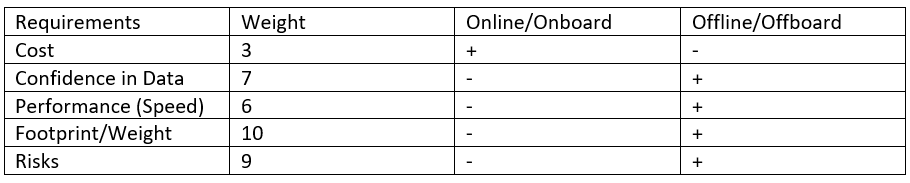
\includegraphics[width=6.21513in,height=1.25in]{Figures/pugh.png}

It's clear that Offline processing offers less risk and more capacity to
achieve what we want, so it is my (Chris) recommendation to go with 2
discrete systems (data acquisition, data processing)

\clearpage \section{GridSearch Attempts}\label{apx:GSAttempt}
This shows how a Grid Search was used for hyperparameter optimisation. In particular, this is an example of an iterative process where the grid was manually narrowed and precision increase. 
\begin{lstlisting}
    parameters={'hidden_layer_sizes': [(145,), (147,), (149,), (151,), (153)],
                'alpha': [0.09, 0.11, 0.13, 0.15, 0.17, 0.19]}
    mlpc = MLPClassifier(verbose=False, early_stopping=True, learning_rate='adaptive',max_iter=1000)
    clf = GridSearchCV(estimator=mlpc, scoring='f1',param_grid=parameters,n_jobs=-1,verbose=1,cv=3);
    clf.fit(X_train,y);
    print(clf.score(X_train, y))
    print(clf.best_params_)
\end{lstlisting}
\begin{lstlisting}
    Fitting 3 folds for each of 30 candidates, totalling 90 fits
    [Parallel(n_jobs=-1)]: Using backend LokyBackend with 4 concurrent workers.
    [Parallel(n_jobs=-1)]: Done  42 tasks      | elapsed:  7.8min
    [Parallel(n_jobs=-1)]: Done  90 out of  90 | elapsed: 14.4min finished
    0.8249400479616308
    {'alpha': 0.11, 'hidden_layer_sizes': (151,)}
\end{lstlisting}


\clearpage \section{Table of ExtraSensory Labels}\label{apx:ExtraSensoryLabels}
\begin{table}[h]
\begin{center}  
\caption{ExtraSensory Labels \cite{Vaizman2017}}\label{tab:ExtraSensoryLabels}
\begin{tabular}{ll}
    \hline\hline
\# & Label Description            \\ \hline 
1  & LYING\_DOWN                  \\
2  & SITTING                      \\
3  & FIX\_walking                 \\
4  & FIX\_running                 \\
5  & BICYCLING                    \\
6  & SLEEPING                     \\
7  & LAB\_WORK                    \\
8  & IN\_CLASS                    \\
9  & IN\_A\_MEETING               \\
10 & LOC\_main\_workplace         \\
11 & OR\_indoors                  \\
12 & OR\_outside                  \\
13 & IN\_A\_CAR                   \\
14 & ON\_A\_BUS                   \\
15 & DRIVE\_-\_I\_M\_THE\_DRIVER  \\
16 & DRIVE\_-\_I\_M\_A\_PASSENGER \\
17 & LOC\_home                    \\
18 & FIX\_restaurant              \\
19 & PHONE\_IN\_POCKET            \\
20 & OR\_exercise                 \\
21 & COOKING                      \\
22 & SHOPPING                     \\
23 & STROLLING                    \\
24 & DRINKING\_\_ALCOHOL\_        \\
25 & BATHING\_-\_SHOWER           \\
26 & CLEANING                     \\
27 & DOING\_LAUNDRY               \\
28 & WASHING\_DISHES              \\
29 & WATCHING\_TV                 \\
30 & SURFING\_THE\_INTERNET       \\
31 & AT\_A\_PARTY                 \\
32 & AT\_A\_BAR                   \\
33 & LOC\_beach                   \\
34 & SINGING                      \\
35 & TALKING                      \\
36 & COMPUTER\_WORK               \\
37 & EATING                       \\
38 & TOILET                       \\
39 & GROOMING                     \\
40 & DRESSING                     \\
41 & AT\_THE\_GYM                 \\
42 & STAIRS\_-\_GOING\_UP         \\
43 & STAIRS\_-\_GOING\_DOWN       \\
44 & ELEVATOR                     \\
45 & OR\_standing                 \\
46 & AT\_SCHOOL                   \\
47 & PHONE\_IN\_HAND              \\
48 & PHONE\_IN\_BAG               \\
49 & PHONE\_ON\_TABLE             \\
50 & WITH\_CO-WORKERS             \\
51 & WITH\_FRIENDS                \\ \hline 
\end{tabular}    
\end{center}
\end{table}


% sounds like dropout is great for making sure accelerometer data is used

% Dropout

% Unlike these methods mentioned above, dropout in my understanding is tricky but practical. Like the figure shown below, the dropout will randomly mute some neurons in the neural network and we therefore have a sparse network which hugely decreases the possibility of overfitting.More importantly, the dropout will make the weights spread over the input features instead of focusing on some features.

% The possibility of muting neurons is often set as 0.5 though you can feel free to make it 0.3 or 1.0. When the dropout is 1.0, then you simply don't drop out any neurons. But our experience tells us 0.5 is usually the best choice.

% ExtraSensory Data BreakdoAfter finishing the training, it is important to turn off the dropout during development and testing. Otherwise, the prediction of this model is not stable since dropout add uncertainties to it.


\end{document}
